% !TeX spellcheck = en_US
%% arara: pdflatex
% arara: pdflatex
% arara: pdflatex
\documentclass[journal,a4paper,10pt,twoside]{IEEEtran} % with epstopdf, add draft=false
\usepackage[utf8]{inputenc}
\usepackage{times,textcomp,amssymb}
\usepackage[cmex10]{amsmath}
\usepackage[T1]{fontenc}
\usepackage[english]{babel}

\usepackage{breqn,cite}
%\usepackage{epstopdf}
\usepackage[dvipsnames]{xcolor}
\usepackage[pdftex]{graphicx}
\usepackage{subfig}
\usepackage[section]{placeins} % floats never go into next section
%\let\labelindent\relax % Compact lists
\usepackage{array,booktabs,enumitem,balance} % nice rules in tables

% amsmath sets \interdisplaylinepenalty = 10000
% preventing page breaks from occurring within multiline equations
\interdisplaylinepenalty=2500

%tikz figures
\usepackage{tikz}
\usetikzlibrary{automata,positioning,chains,shapes,arrows}
\usepackage{pgfplots}
\usetikzlibrary{plotmarks}
\newlength\fheight
\newlength\fwidth
\pgfplotsset{compat=newest}
\pgfplotsset{plot coordinates/math parser=false}

\newcommand{\EB}[1]{\textit{\color{blue}EB says: #1}}
\newcommand{\FR}[1]{\textit{\color{ForestGreen}FR says: #1}}
\newcommand{\LA}[1]{\textit{\color{orange}LA says: #1}}
\newcommand{\FS}[1]{\textit{\color{red}FS says: #1}}

\usepackage{hyperref}
\definecolor{dkpowder}{rgb}{0,0.2,0.7}
\hypersetup{%
    pdfpagemode  = {UseOutlines},
    bookmarksopen,
    pdfstartview = {FitH},
    colorlinks,
    linkcolor = {dkpowder},
    citecolor = {dkpowder},
    urlcolor  = {dkpowder},
}

\pdfminorversion=7 % fixes warnings of eps to pdf included images

%%%%%%%%%%%%%%%%
\begin{document}
\title{On the Iterated Prisoner's Dilemma}

\author{%
    \IEEEauthorblockN{Elia Bonetto, Filippo Rigotto, Luca Attanasio and Francesco Savio}

    \IEEEauthorblockA{Department of Information Engineering, University of Padova -- Via Gradenigo, 6/b, 35131 Padova, Italy}
    % \\Email: {\tt\{bonettoe,rigottof,attanasiol,\}@dei.unipd.it}}
}

\maketitle
%%%%%%%%%%

\begin{abstract}
In this work we analyse the Iterated Prisoner's Dilemma (IPD), in different scenarios: between two players, between multiple players, between multiple players with evolving population and between multiple players with a random gene between rounds representing the grade of cooperation (a Nature choice, in Game Theory terms).
At first this report gives an introduction on the Prisoner's Dilemma problem theoretically and mathematically, then it defines a base structure that will be used in all the following section.
In Section~\ref{s:str} we illustrate the possible strategies that have been implemented in this work, in Sections [\ref{s:IPD2P}, \ref{s:IPDMP}, \ref{s:rIPDMP}, \ref{s:crIPDMP}] the results of the simulations are presented for each study-cases.
At the end, in Section~\ref{s:conc}, some final thoughts and considerations are presented concluding the work.
All the code, developed in \textit{Python 3.7}, can be found on \href{https://github.com/eliabntt/LaboratoryOfComputationalPhysics/tree/Group9}{GitHub}.
\end{abstract}

\section{Introduction} 
The Prisoner's Dilemma (PD) is a classical game analyzed in Game Theory which attempts to model social and economical interactions. It is a \textit{dilemma} because, if exploited to explain the emergence of altruism in human or in general in animal society, it fails badly at a first glance. As we will see shortly, if the intuition tells us that the best choice is to cooperate the only stable point and win-ever strategy in a one-shot game is to \textit{not} cooperate.

The classical formulation of the PD is that given two prisoners in a scenario where their conviction depends on their mutual cooperation, they can either stay silent or fink, respectively cooperate or defect (not cooperate). 
Another possible formulation is by the means of a trade-off game called \textit{closed bag exchange}:

\begin{quote}
\textit{Two people meet and exchange closed bags, with the understanding that one of them contains money, and the other contains a purchase. Either player can choose to honor the deal by putting into his or her bag what he or she agreed, or he or she can defect by handing over an empty bag.}
\end{quote}

Mathematically the PD can be expressed with linear algebra. The key component is the \textit{Payoff matrix} $M$, which quantifies the reward of each player depending on whether he/she cooperated or defect:

$$
M = 
\begin{pmatrix} 
R & S \\
T & P 
\end{pmatrix}
$$

where $T$ (Temptation), $R$ (Reward), $S$ (``Sucker's''), $P$ (Punishment) are integers that satisfy the following conditions:

$$
T>R>P>S; \quad 2R > T+S 
$$
For example, $T=3$, $R=2$, $P=1$ and $S=0$.
%, or  $T=5$, $R=3$, $P=2$, $S=0$. 

$R$ is given if both cooperates, $S$ if who's watching the matrix cooperate and the other defect, $T$ is the opposite of $S$ and finally $P$ is if both players defect.

As for the representation of the game for a single round, each player's choice (move) can be represented by one of the two axis in $\mathbb{R}^2$, i.e. $u_C=\begin{pmatrix} 1 \\ 0 \end{pmatrix}$ or $u_D=\begin{pmatrix} 0 \\ 1 \end{pmatrix}$, where the first coordinate stands for \textit{Cooperate} and the second for \textit{Defect}. Being $u_1$ and $u_2$ the moves of the first and second player respectively, their rewards $r_1$ and $r_2$ can then be computed as:

$$
r_1 = u_1^T M u_2
\quad
\quad
r_2 = u_2^T M u_1
$$

For a single-shot game (a game which is played only once), the best strategy (choice of action) may seem for both players to cooperate as this leads to a good payoff which maximizes the global outcome, evaluated as the sum of the payoffs for each of them. This is indeed the \textit{Pareto dominating strategy}. 

However if a player cooperates, he has an incentive to deviate from his choice and so to betray the other player and defect as this leads to a better payoff for himself, and this is true for both players. 
Given the fact that both players are rational and fully aware of the rules of the game (they have \textit{common knowledge}, using Game Theory terms) and that they move simultaneously, both of them will easily conclude that the best way of acting is to defect as this would lead to a slightly lower payoff if the opponent defects (minor punishment) but a higher one if the other player chooses to cooperate.
Following this, the only possible reasonable conclusion is that the only \textit{Nash Equilibrium}, or the only way to win this game in a single-shot scenario, is to always defect.
This is not \textit{Pareto optimal} but playing cooperate, as we have just seen, is not feasible: the only strategy in which nobody wants to deviate is to defect.

This reasoning is no longer true when we consider repeated games and in particular the Iterated Prisoner Dilemma (IPD) since the IPD involves time and memory (history). In addition, more complicated strategies can be introduced like random strategies, grim triggers or Tit For (Two) Tat.
Winning a game in this setup means to achieve a better payoff in the long run. In Section~\ref{s:IPD2P} we will see a simple one-vs-one game, iterated through time, while in the subsequent cases population and other dynamics will be involved.

\section{Strategies} \label{s:str}
The strategy is represented as a function which outputs either $u_C$ or $u_D$. Depending on the strategy, such function might depend on one or both players' history of moves, or on the number of moves played till that moment and so on.
The strategy is based on a probability density function. In this project we used both strategies based on probability and deterministic ones.

The strategies based on probability are:

\begin{description}
    \item[Nice guy] always cooperate (function's output is always $u_C$).
    \item[Bad guy] always defect (function's output is always $u_D$).
    \item[Indifferent] randomly defect half $(k=50\%)$ of the times.
    \item[Mainly nice] randomly defect $k\%$ of the times, $k<50$.% and cooperate $100-k\%$, with $k<50$.
    \item[Mainly bad] randomly defect $k\%$ of the times, $k>50$.% and cooperate $100-k\%$, with $k>50$.
\end{description}

The deterministic strategies are:
\begin{description}
    \item[Tit-for-Tat (TfT)] start by cooperating the first time, then repeat opponent's previous move.
    \item[Tit-for-Two-Tat (Tf2T)] start by cooperating the first two times, then defect only if the opponent defected last two times.
    \item[Grim-Trigger (GrT)] always cooperate until the opponent's first defect move, then always defect. 
\end{description}

These strategies are fixed in time, i.e. a player cannot change the strategy it was created with, except in the last cases, examined in Section~\ref{s:crIPDMP}.

\section{Two players IPD} \label{s:IPD2P}
In this section the IPD intercourse between two players: each player has a strategy, does not know the strategy of the opponent and plays accordingly to his strategy definition without possibility to change it. This game is repeated for a fixed number of rounds, unknown to the two players. The main metric out of this game is who wins, or in other words who achieves a higher payoff at the end of the round.

We fixed the number of iterations to \texttt{NUM\_ITER = 50}. This could also be seen as the number of moves during the match, and can be changed, but the results does not depends on it in most of the cases (the only exceptions could be the random ones).

All the possible combinations between players are evaluated, including the case of the player playing against itself.
This is a simple repetition of the single-shot game with the addition of memory and the possibility to add, as we have already seen, probabilistic and more elaborated strategies.

Since we are not concerned about population in this case (it is a simple A vs B game), as expected the winning strategy in all cases is to \textit{not} cooperate, or, in other terms, the \textit{Always Bad guy} strategy. 

In fact in all cases \textit{Bad guy} has a higher reward than the opponent as in Figures~[\ref{fig:badvstft}, \ref{fig:badvsnice}, \ref{fig:badvsmainlybad}]. 
On the other hand, when \textit{Bad guy} plays against \textit{Bad guy} as in \autoref{fig:badvsbad}, or similarly against \textit{Mainly bad}(\autoref{fig:badvsmainlybad}), this leads to the same cumulative reward for both players or almost the same respectively, but not as good as if they were playing against (mainly) nice strategies. This is a first important insight that verifies and points out what we have seen only theoretically before: defect is always a winning strategy, but it may be non-optimal; on the other hand if both are playing cooperate, each one of them would get an advantage if they defect against the other.

\begin{figure}[!ht]
    \centering
    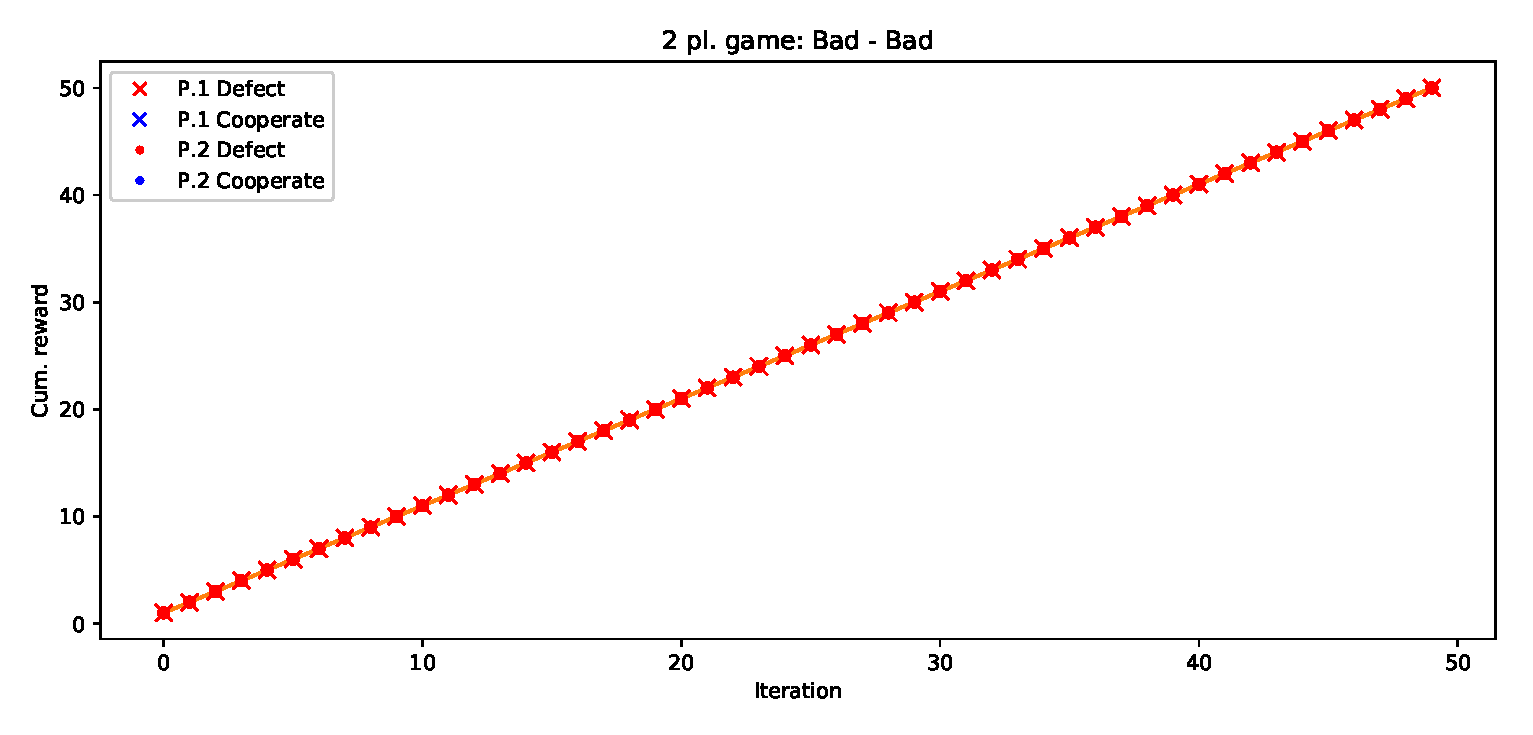
\includegraphics[width=1\columnwidth]{../img/ipd2p/ipd2p-rewards-Bad-Bad}
    \caption{Bad vs Bad}
    \label{fig:badvsbad}
\end{figure}

\begin{figure}[!ht]
    \centering
    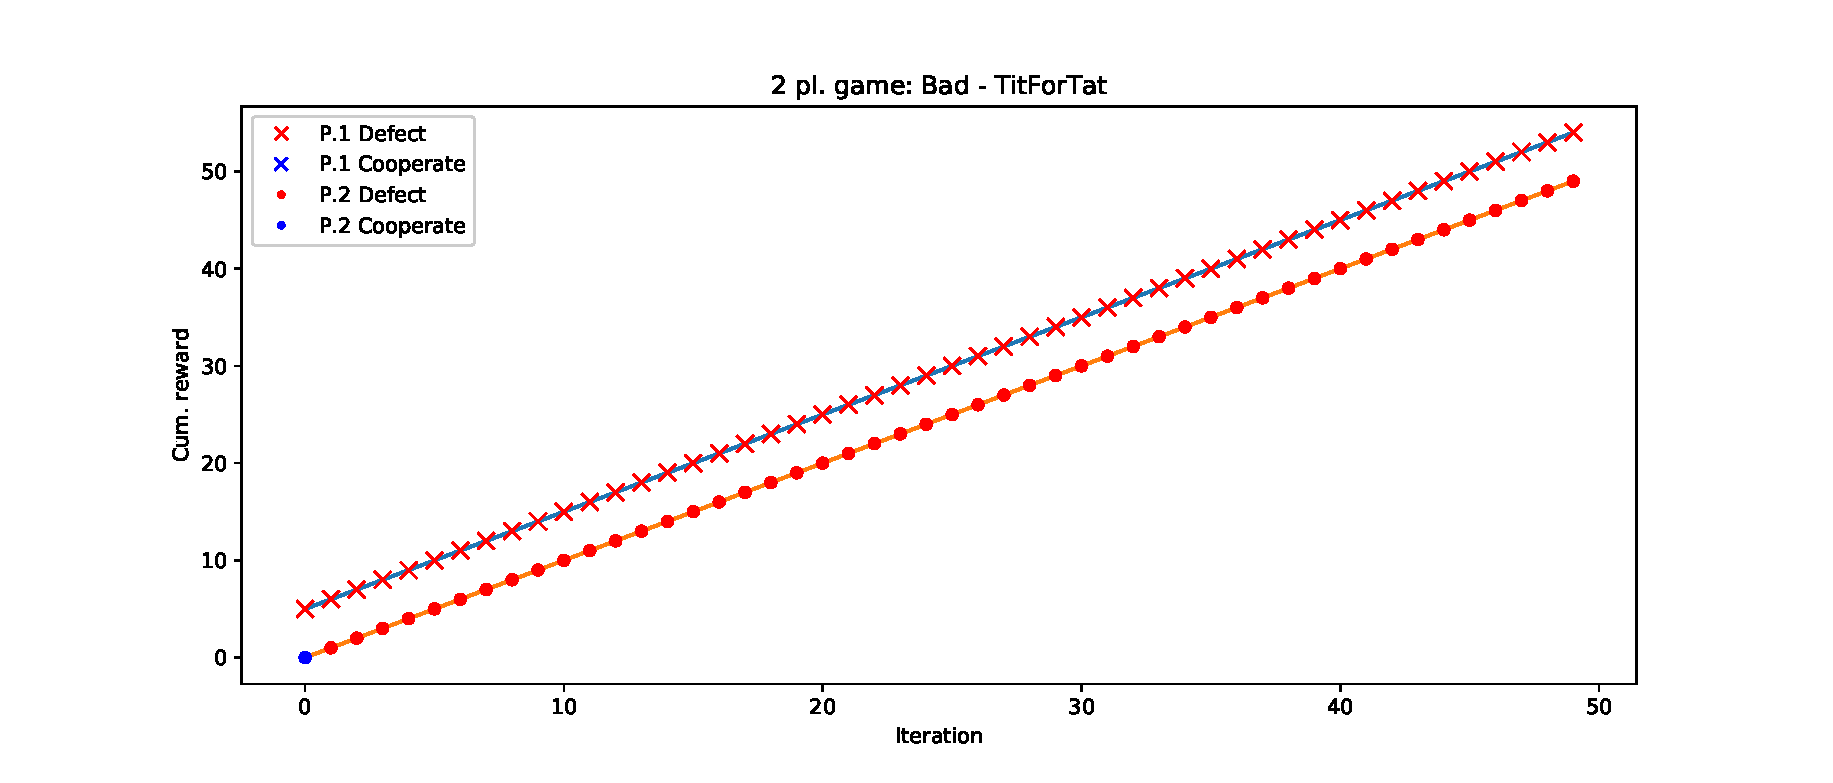
\includegraphics[width=1\columnwidth]{../img/ipd2p/ipd2p-rewards-Bad-TitForTat}
    \caption{Bad vs TfT}
    \label{fig:badvstft}
\end{figure}

\begin{figure}[!ht]
    \centering
    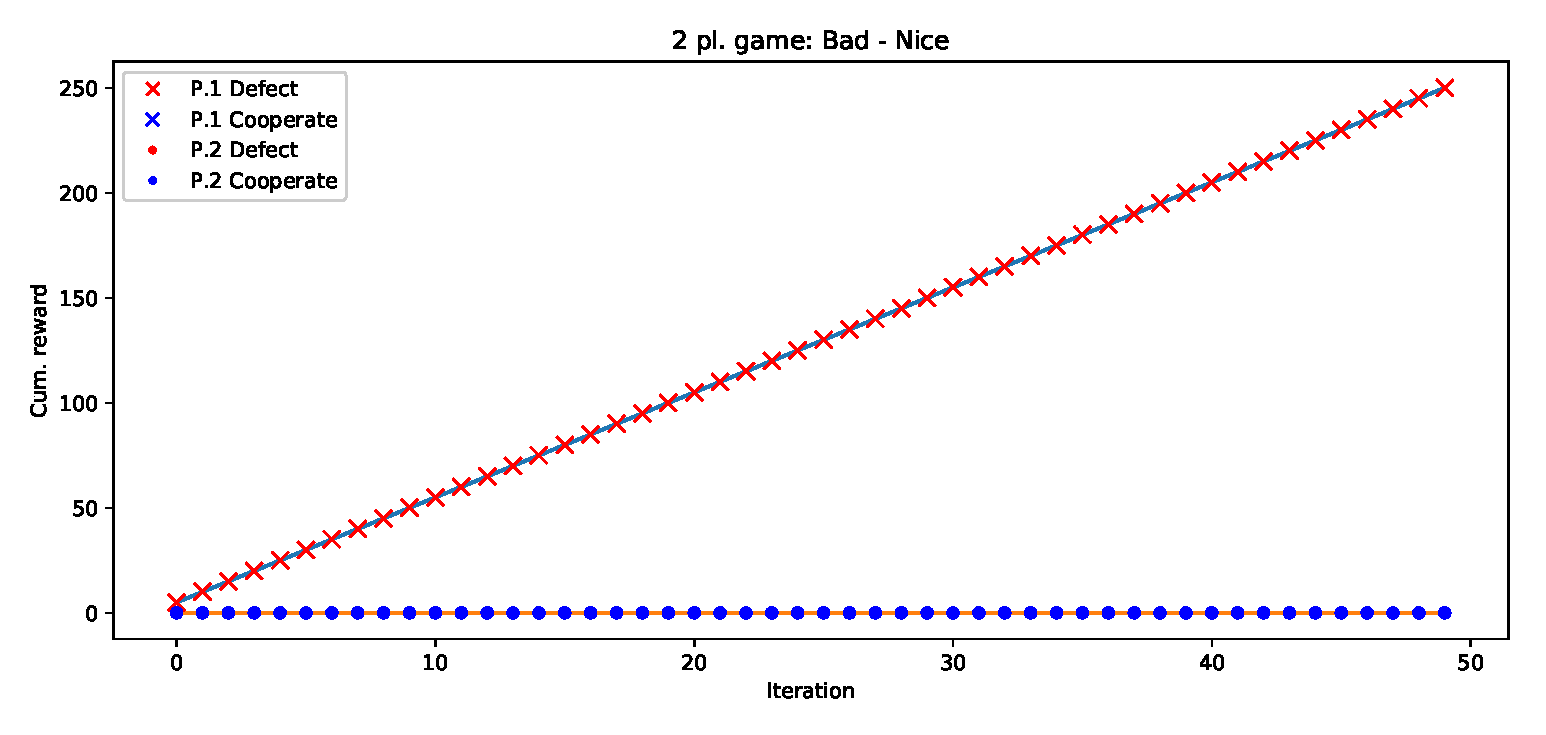
\includegraphics[width=1\columnwidth]{../img/ipd2p/ipd2p-rewards-Bad-Nice}
    \caption{Bad vs Nice}
    \label{fig:badvsnice}
\end{figure}

\begin{figure}[!ht]
    \centering
    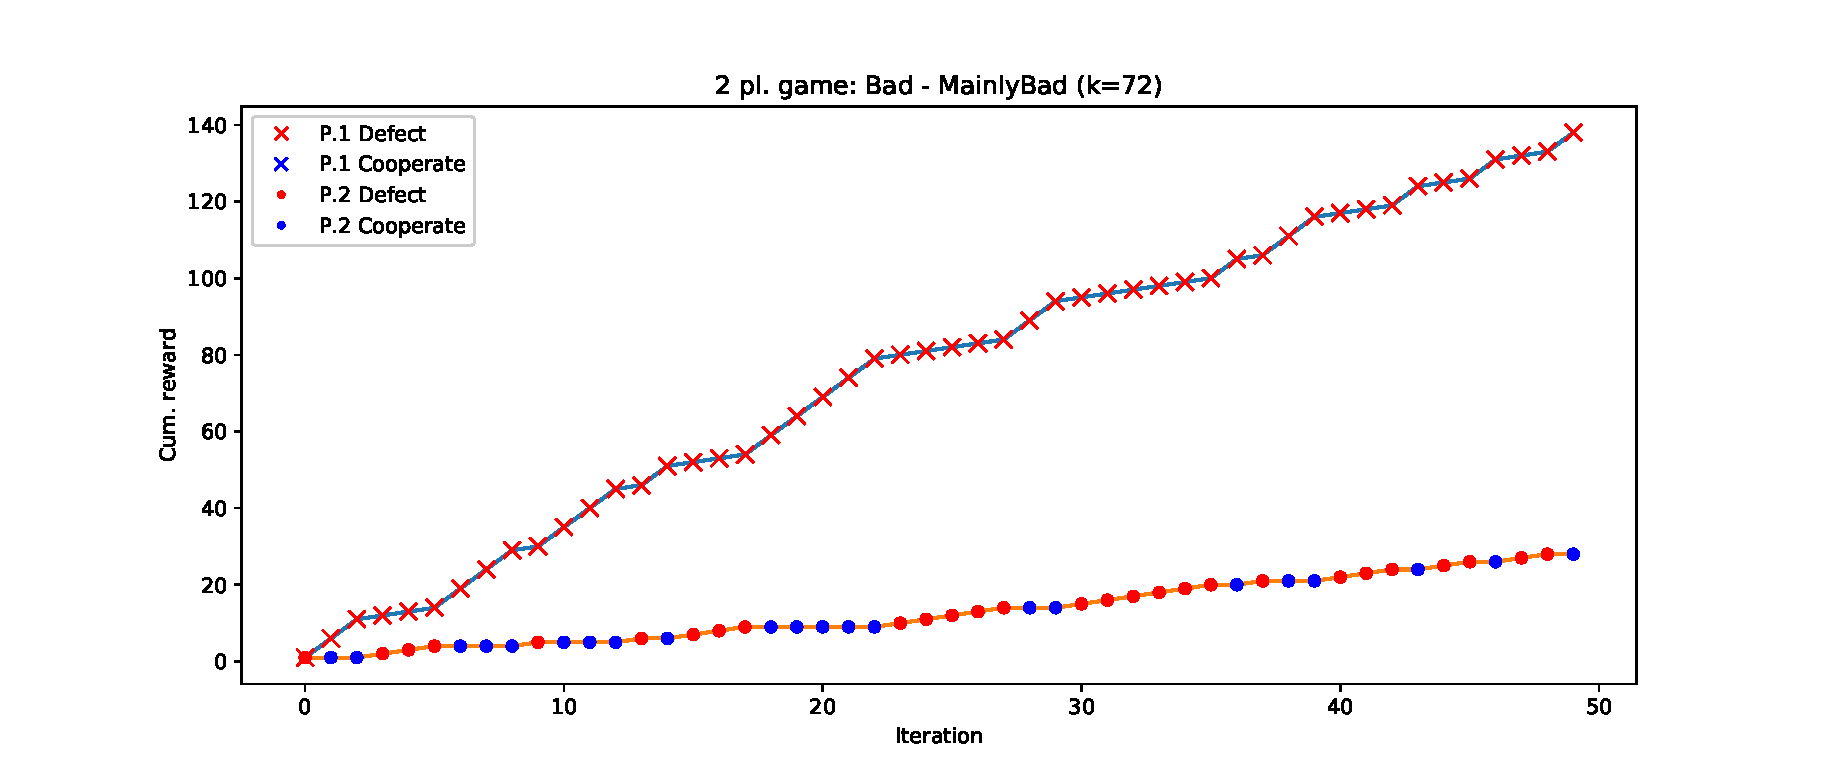
\includegraphics[width=1\columnwidth]{../img/ipd2p/ipd2p-rewards-Bad-MainlyBad(k=72)}
    \caption{Bad vs Mainly bad}
    \label{fig:badvsmainlybad}
\end{figure}

If we take a closer look, the combination of \textit{Nice} and one between \textit{TfT} or \textit{Nice} leads to better payoffs at the end of the run as in Figures~[\ref{fig:tftvsindiff}, \ref{fig:nicevsnice}, \ref{fig:nicevstft}]. The concept is both player getting the highest reward, not just one of them, in that case it would be the \textit{Bad}-\textit{Nice} combination. These are isolated cases that we are considering just because it is a study case since the only strategy that wins against all the others and draw with itself is the \textit{Bad} one and so this is the strategy one intelligent player should go for(remember the base-rule that we do not know the strategy of the player we are facing).

\begin{figure}[!ht]
    \centering
    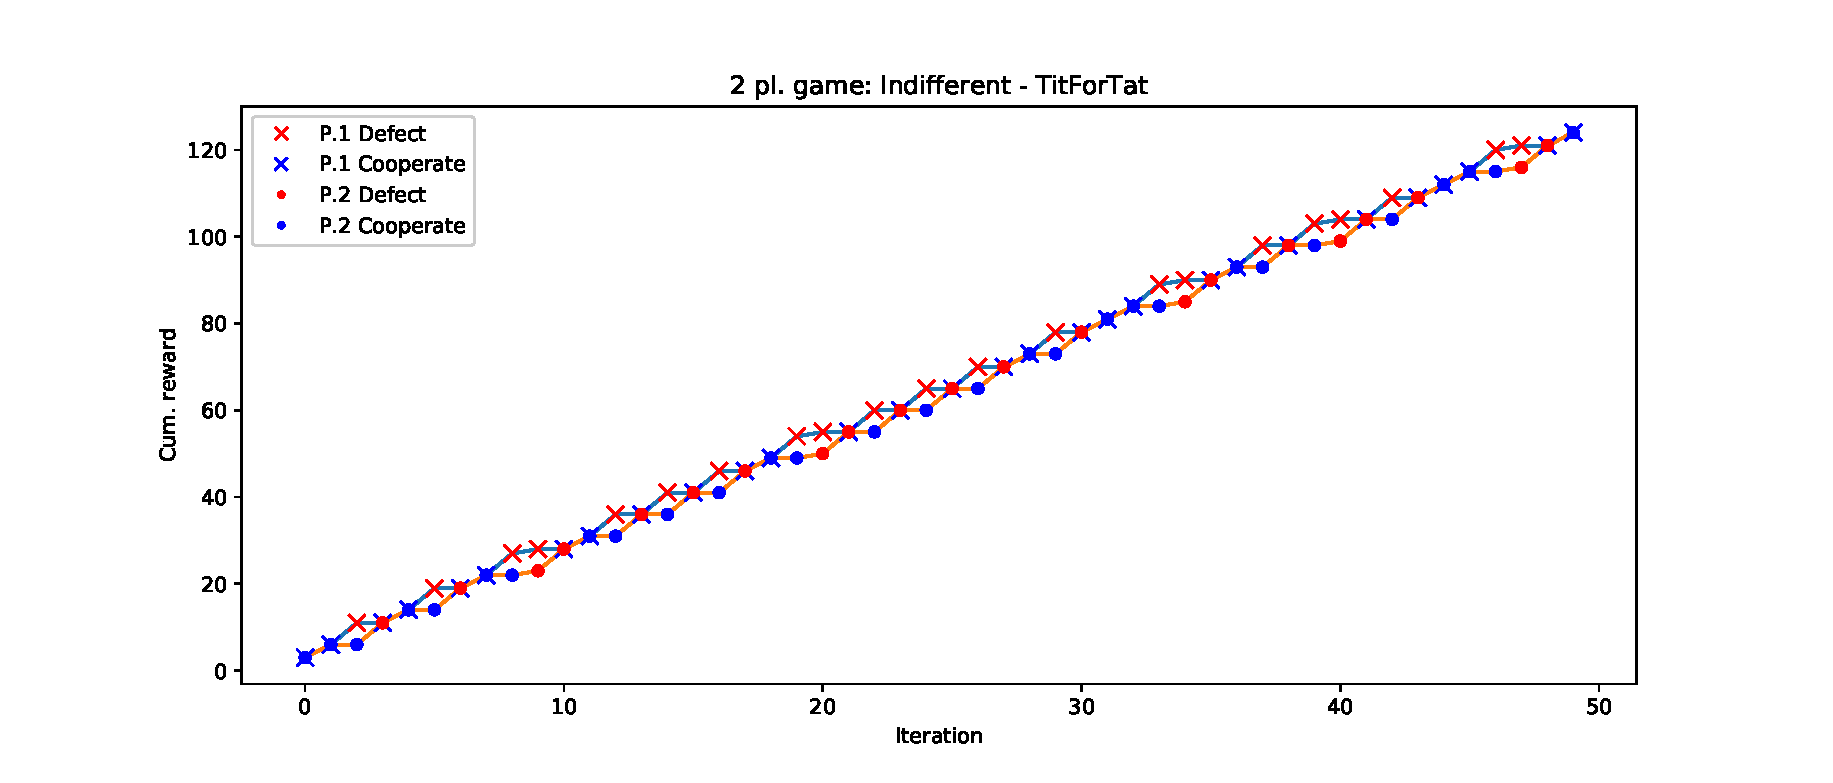
\includegraphics[width=1\columnwidth]{../img/ipd2p/ipd2p-rewards-Indifferent-TitForTat}
    \caption{TfT vs Indifferent}
    \label{fig:tftvsindiff}
\end{figure}

\begin{figure}[!ht]
    \centering
    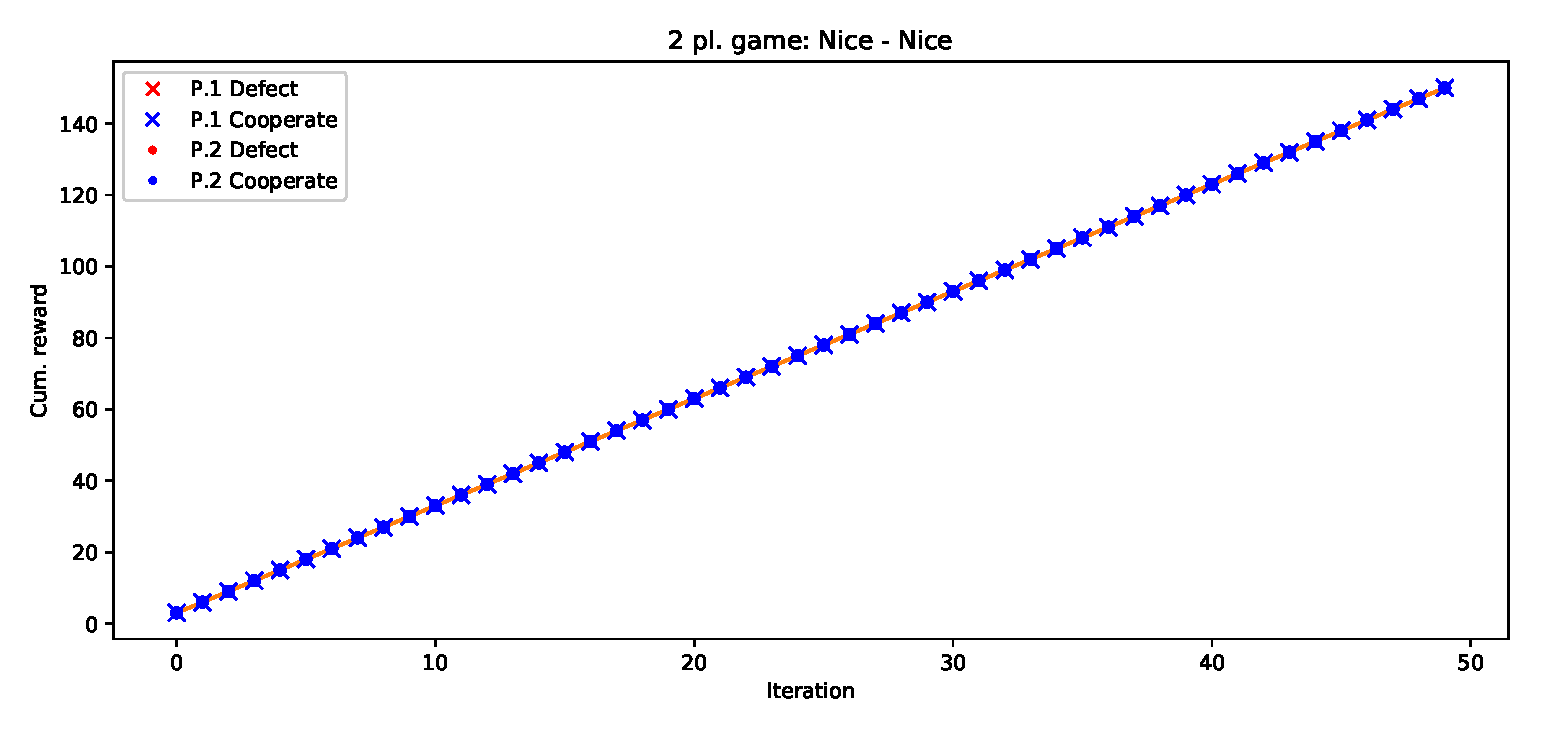
\includegraphics[width=1\columnwidth]{../img/ipd2p/ipd2p-rewards-Nice-Nice}
    \caption{Nice vs Nice}
    \label{fig:nicevsnice}
\end{figure}

\begin{figure}[!ht]
    \centering
    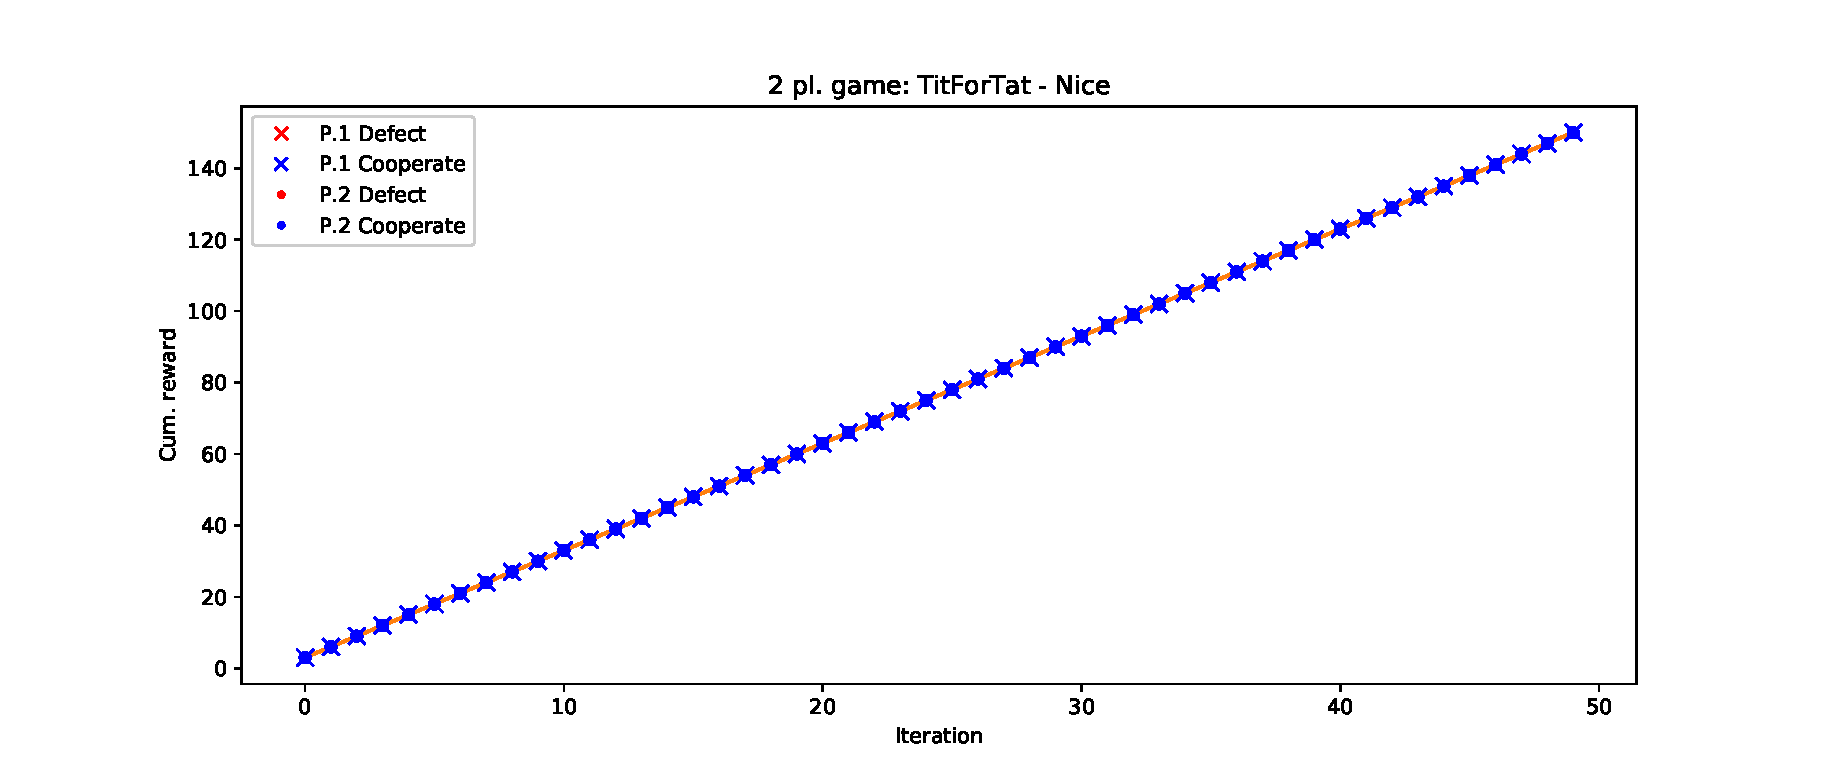
\includegraphics[width=1\columnwidth]{../img/ipd2p/ipd2p-rewards-TitForTat-Nice}
    \caption{Nice vs TfT}
    \label{fig:nicevstft}
\end{figure}

\begin{figure}[!ht]
    \centering
    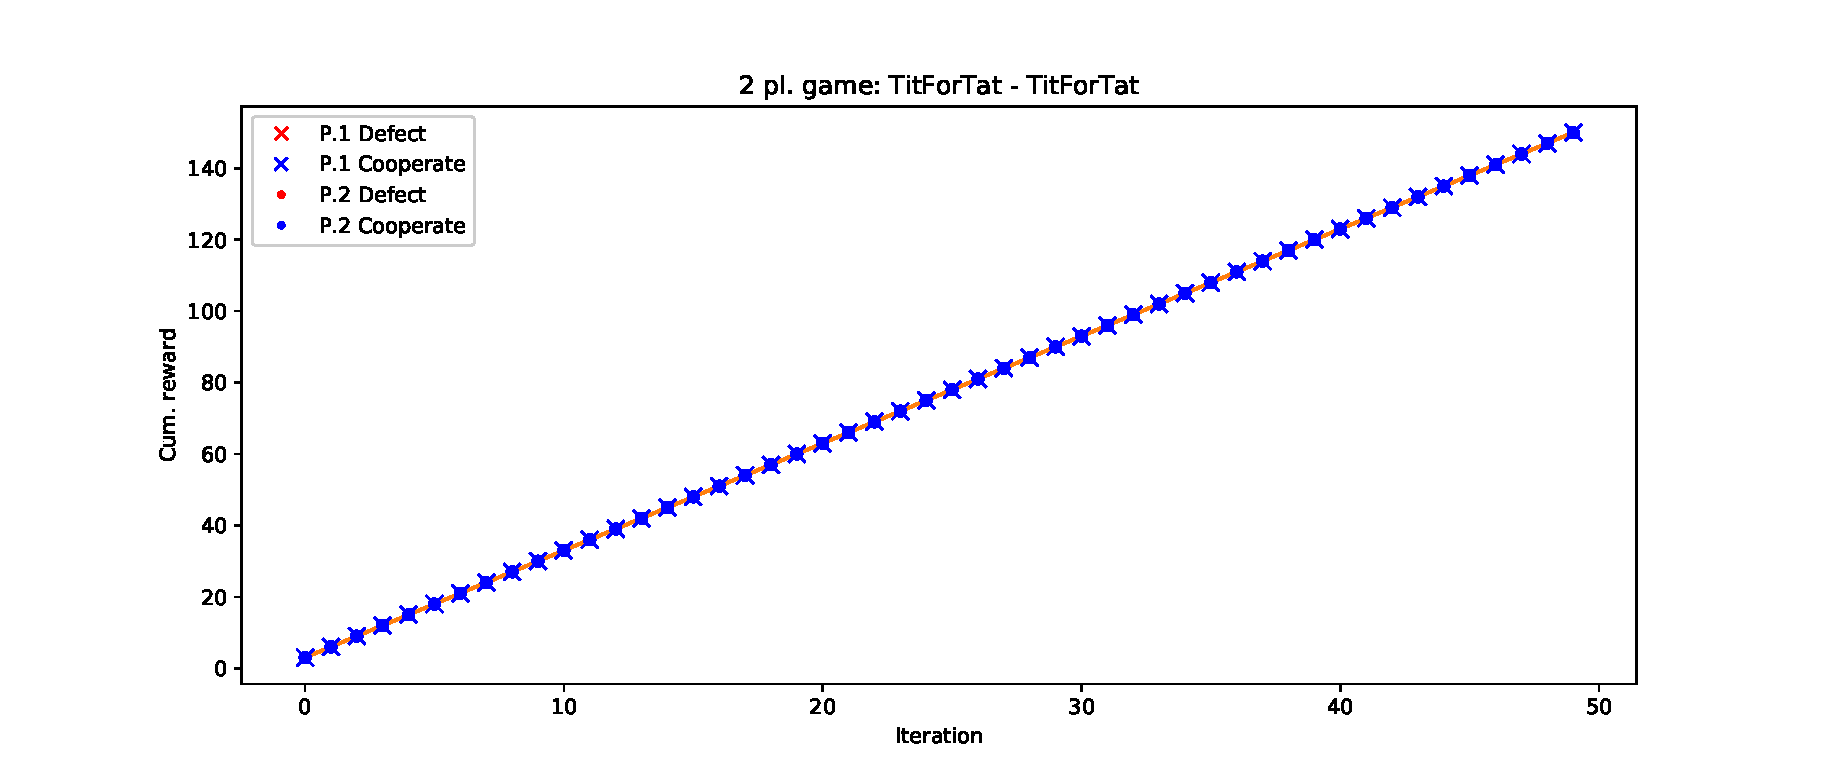
\includegraphics[width=1\columnwidth]{../img/ipd2p/ipd2p-rewards-TitForTat-TitForTat}
    \caption{TfT vs TfT}
    \label{fig:tftvstft}
\end{figure}

The TfT strategy is interesting, because TfT leads to almost the same cumulative reward as the opponent, and it is highly adaptive, even if fast-forgivin if it encouter a mainly bad strategy. 
A player might choose this move if he/she wants almost the same reward as the opponent. This strategy will become more insteresting in the following steps.


In addition to this considerations we have run the simulation multiple times to get insight of mean and variances that rule these games. Obviously the static strategies(as the \textit{Nice-Nice} \ref{fig:box-nn}), or the non-triggering ones, or the the ones without variation have constant mean and $0$ std. What is interesting though is for the random ones as we can see that the results can vary quite a bit(as \textit{Mainly Bad-TitForTat}\ref{fig:boxmbvtft}).

\begin{figure}[!ht]
    \centering
    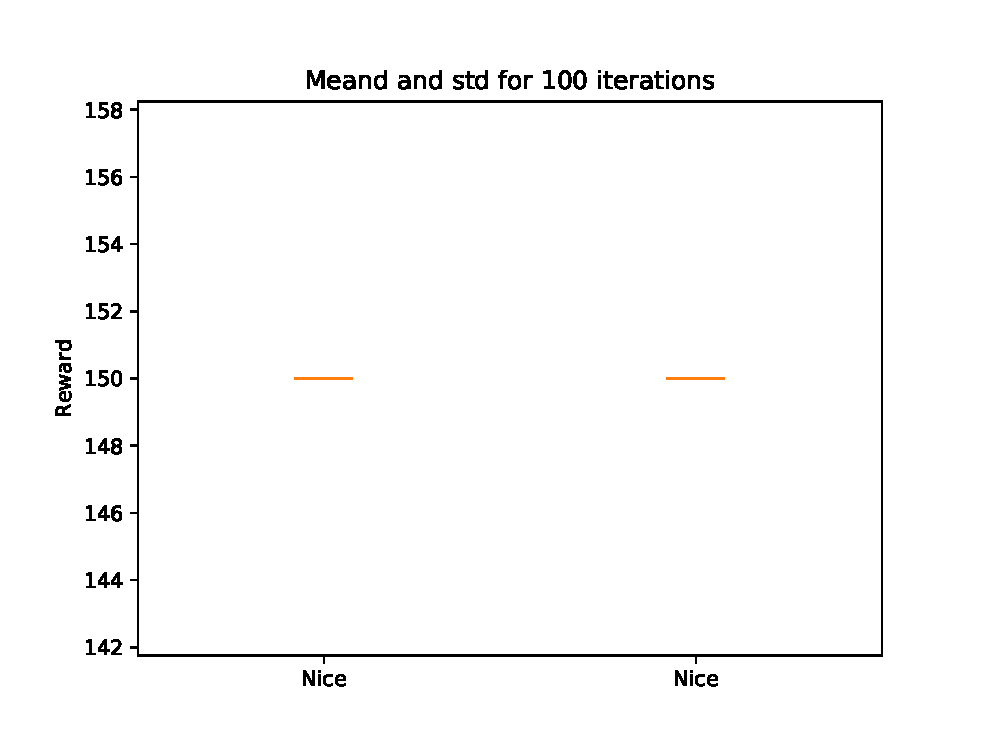
\includegraphics[width=1\columnwidth]{../img/ipd2p/ipd2p-boxplot-Nice-Nice}
    \caption{Nice vs Nice}
    \label{fig:boxnn}
\end{figure}

\begin{figure}[!ht]
    \centering
    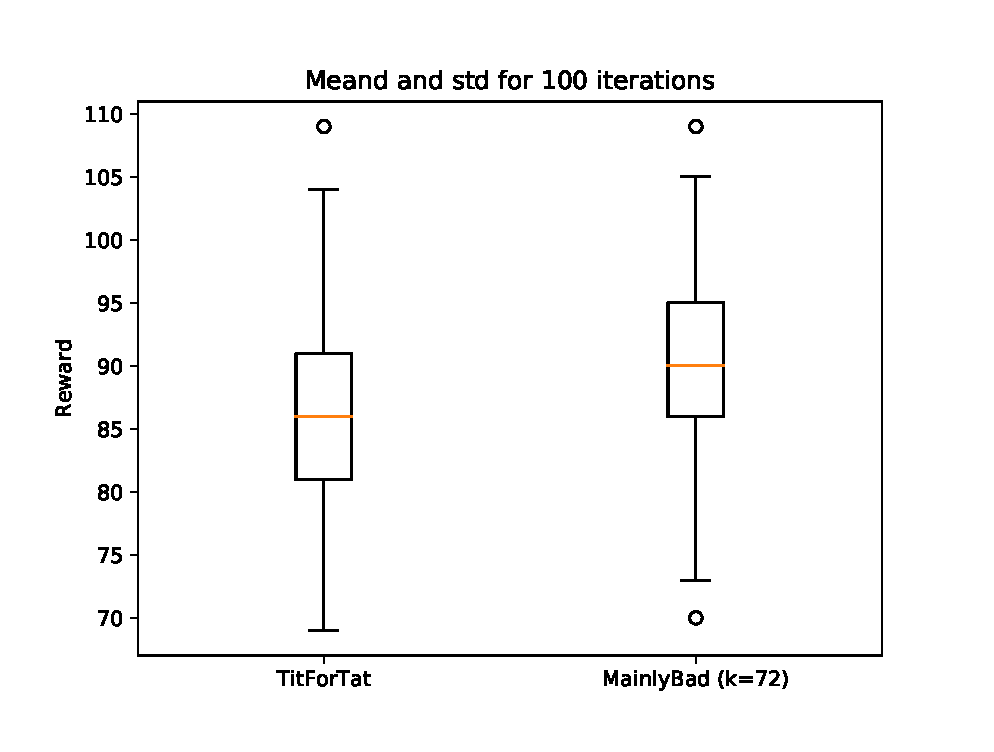
\includegraphics[width=1\columnwidth]{../img/ipd2p/ipd2p-boxplot-TitForTat-MainlyBad(k=72)}
    \caption{TfT vs Mainly Bad}
    \label{fig:boxmbvtft}
\end{figure}

If you want to have more insights about this part, the complete collection of the generated pictures can be found in the repository and in the table \ref{} statistics and results. We can see that the only strategies that reach $0$ as final payoff are the \textit{Nice} ones, while the \textit{TfT, Tf2T, GrT. Bad} have an higher minimum value.
\textbf{INSERT TABLE HERE}


\section{Multiple players IPD - Round-robin scheme} \label{s:IPDMP}
The IPD with \textit{round-robin} (RR) scheme, used to match-up the opponents, consists in a number of players, with various strategies, not necessarily different, each player playing once against each other for a \texttt{NUM\_ITER = 50} of times. 

Each player chooses its fixed strategy at the beginning of the tournament and holds it throughout the course of the whole procedure and nobody knows the strategies of the other players.

In short it is a variation of the previous case, considering multiple players and not just two, playing in a RR way. The single player will win if at the end of the tournament he has the highest cumulative payoff. The culumative points after each match are shown in \autoref{fig:mpipd20}.

\begin{figure}[!ht]
    \centering
    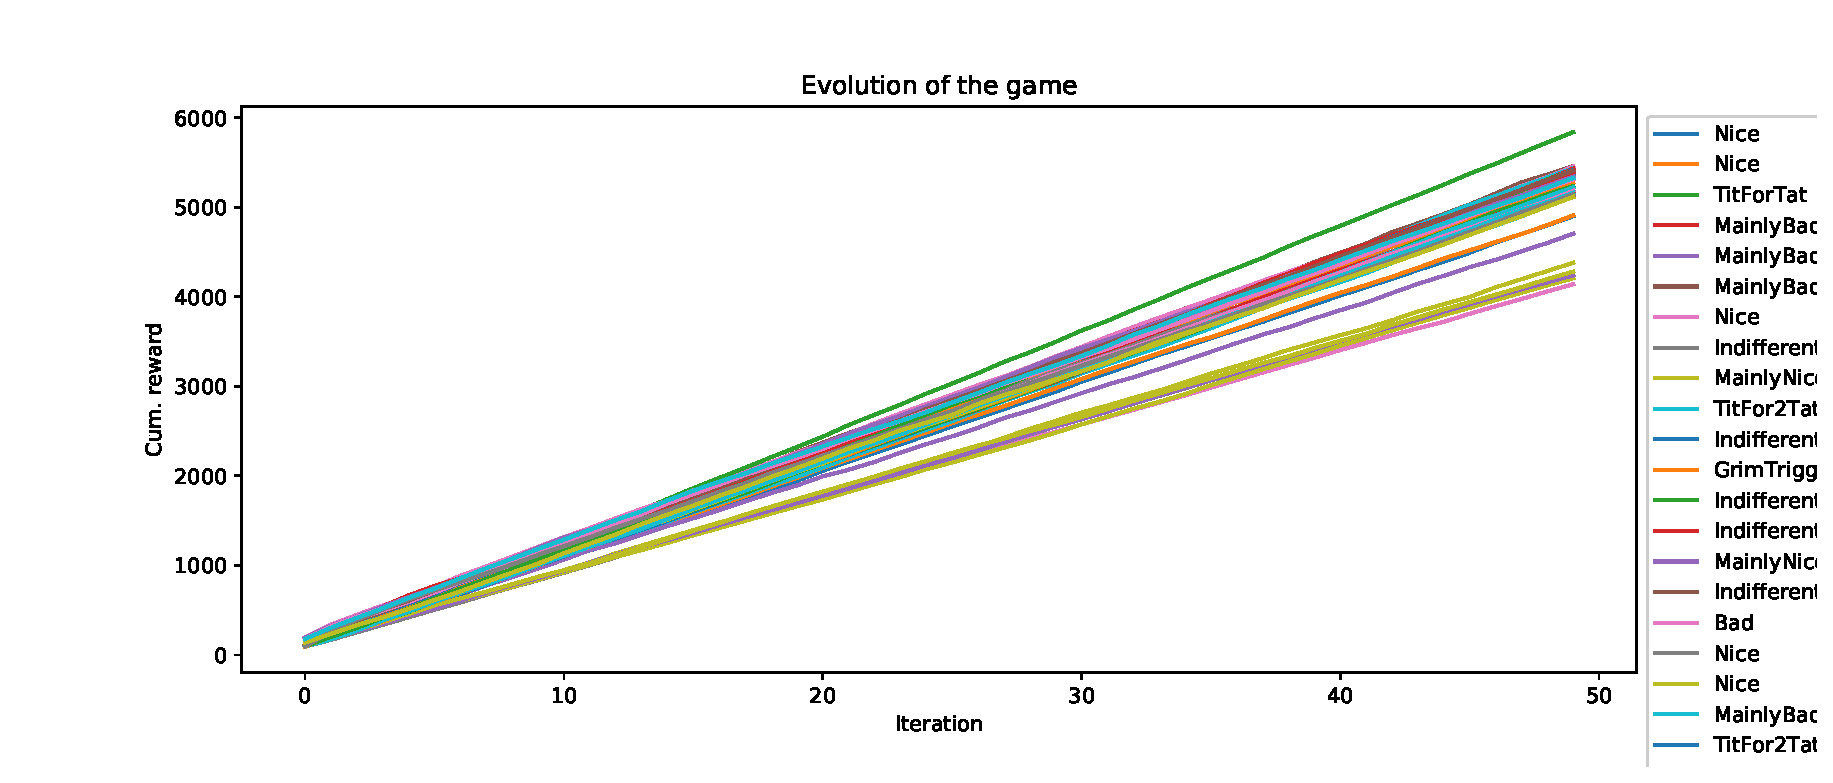
\includegraphics[width=1\columnwidth]{../img/ipdmp/ipdmp-evolution-of-game-50}
    \caption{Boxplot IPDMP}
    \label{fig:boxIPDMP}
\end{figure}

\begin{figure}[!ht]
    \centering
    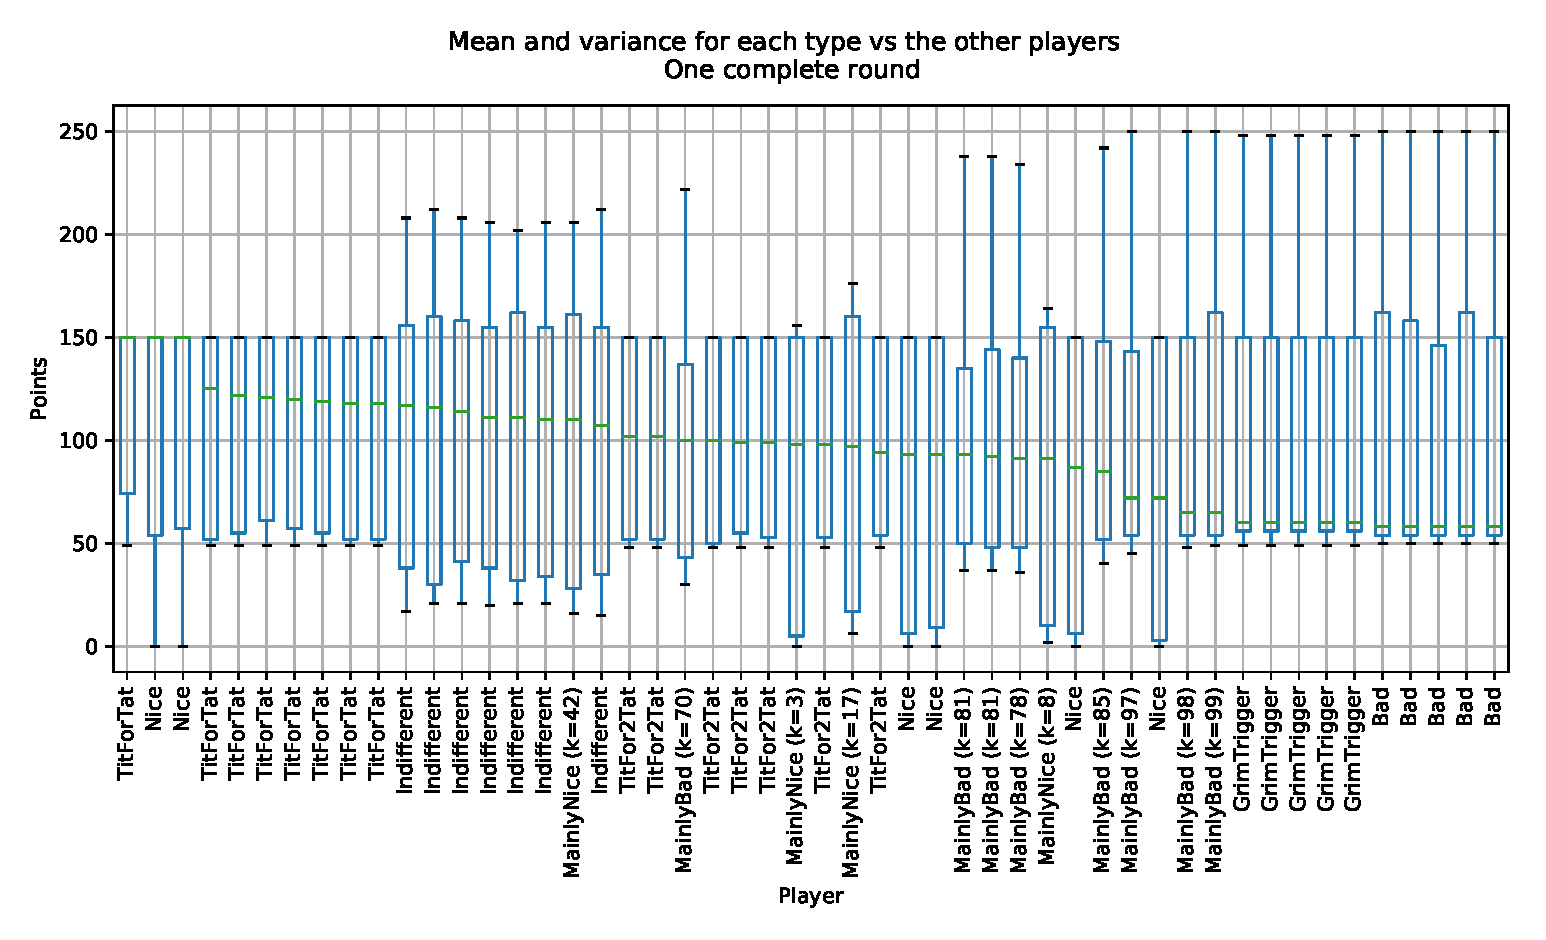
\includegraphics[width=1\columnwidth]{../img/ipdmp/ipdmp-boxplot-single-match-50}
    \caption{Boxplot IPDMP}
    \label{fig:boxIPDMP}
\end{figure}

\begin{figure}[!ht]
    \centering
    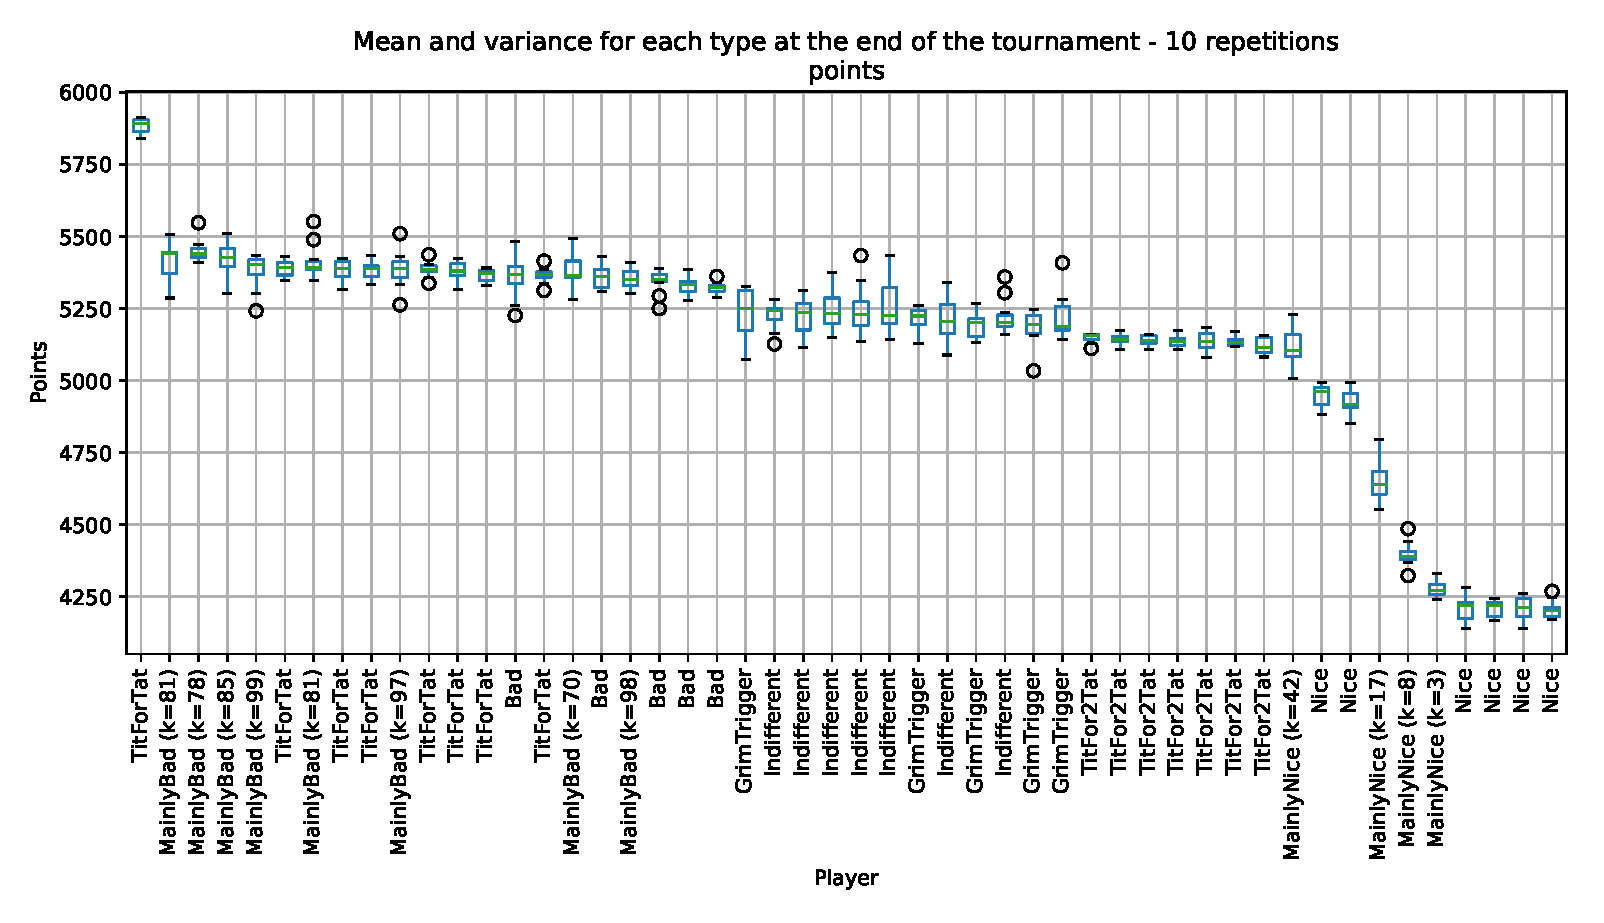
\includegraphics[width=1\columnwidth]{../img/ipdmp/ipdmp-boxplot-final-points-50}
    \caption{Boxplot IPDMP}
    \label{fig:boxIPDMP}
\end{figure}

The outcome of each match of the tournament can be seen in \autoref{tab:match_df}. \FR{table placeholder here}

The results of this game(and of the following cases) depends on the initial population and the balance between \textit{Bad} and \textit{TfT} players. The best strategy overall seems to be the \textit{TfT} one \textbf{ADD CITATION}.

Even in this case we can see variations of the results obtained by running the simulation multiple times and generating the boxplots. As we can see there is no doubt who would win the match \textbf{with the given population}.

\textbf{ADD TABLE}

\section{Repeated multiple players IPD - RR scheme} \label{s:rIPDMP}
We then used the previuosly defined MPIPD round-robin scheme tournament, iterating it many times to collect more advanced statistics.
We identify this as a \textit{Repeated multiple players IPD} (rMPIPD).

We have developed three separated simulations to study the behaviour of the populations and the convergence speed. A population is said to be converged if more than $3/4$ of it has the same type at the end of a complete round. The base rules are the same(common knowledge, strategy unknown to the other players...).

\subsection{Static Population}
In this case we fixed a number of players, each one with a strategy that has the same probability of the other ones. At the end of each round the first third of the population is doubled(the third that achieves the highest cumulative payoff), and the last third is eliminated. In this way we can ensure a static total number of players and study the convergence of the population.
We can easily see how the \textit{TfT} strategy outpaces the other in a very fast way. In requires only $4$ iterations to overcome the other strategies.

\begin{figure}[!ht]
    \centering
    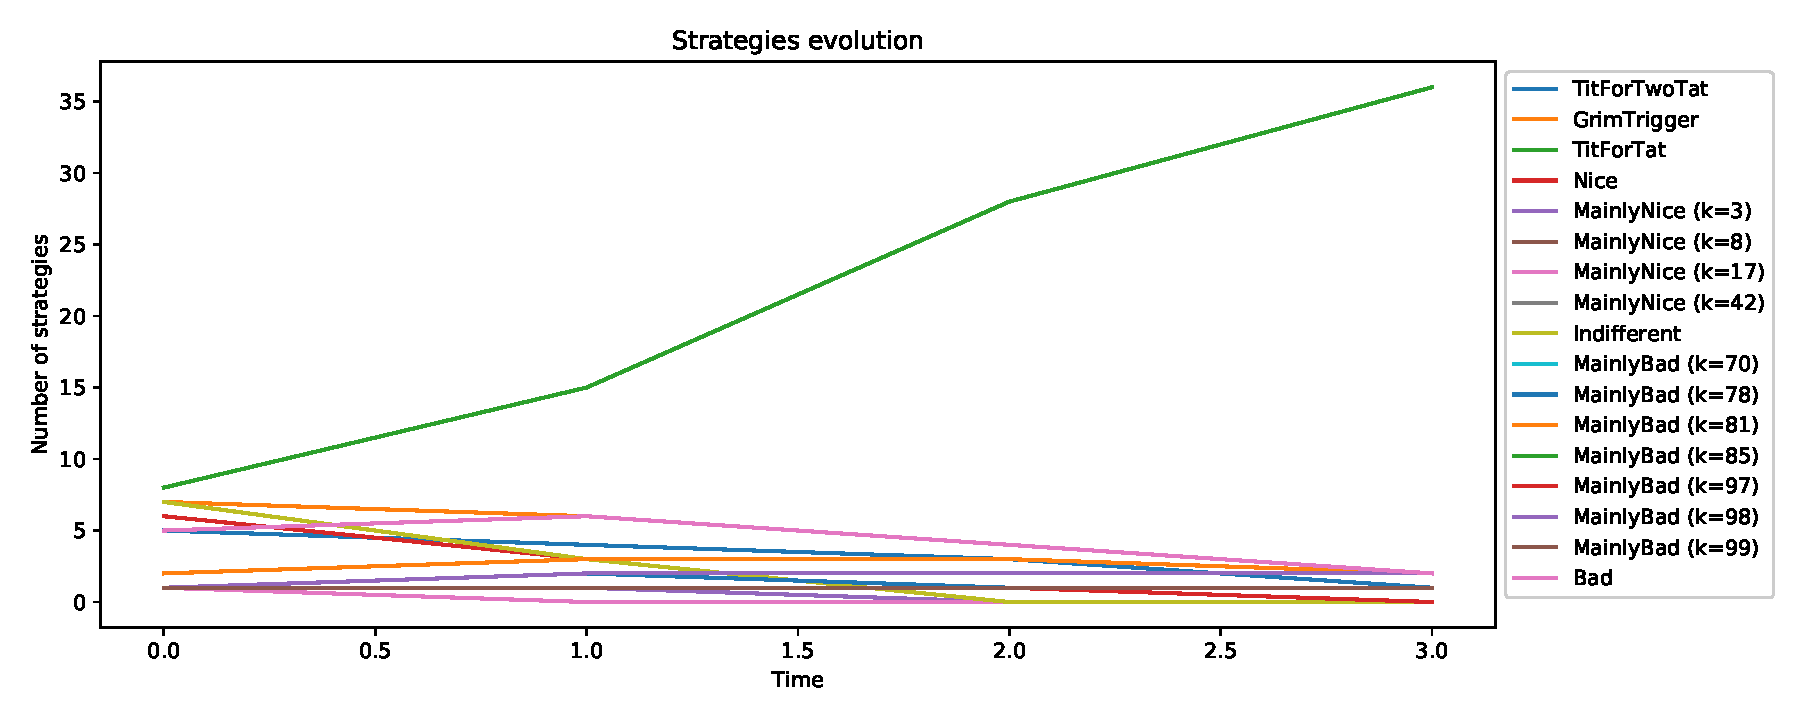
\includegraphics[width=1\columnwidth]{../img/ripdmp-const/ripdmp-evolution-const-pop-50}
    \caption{Evolution RIPDMP constant population}
    \label{fig:constR}
\end{figure}

\begin{figure}[!ht]
    \centering
    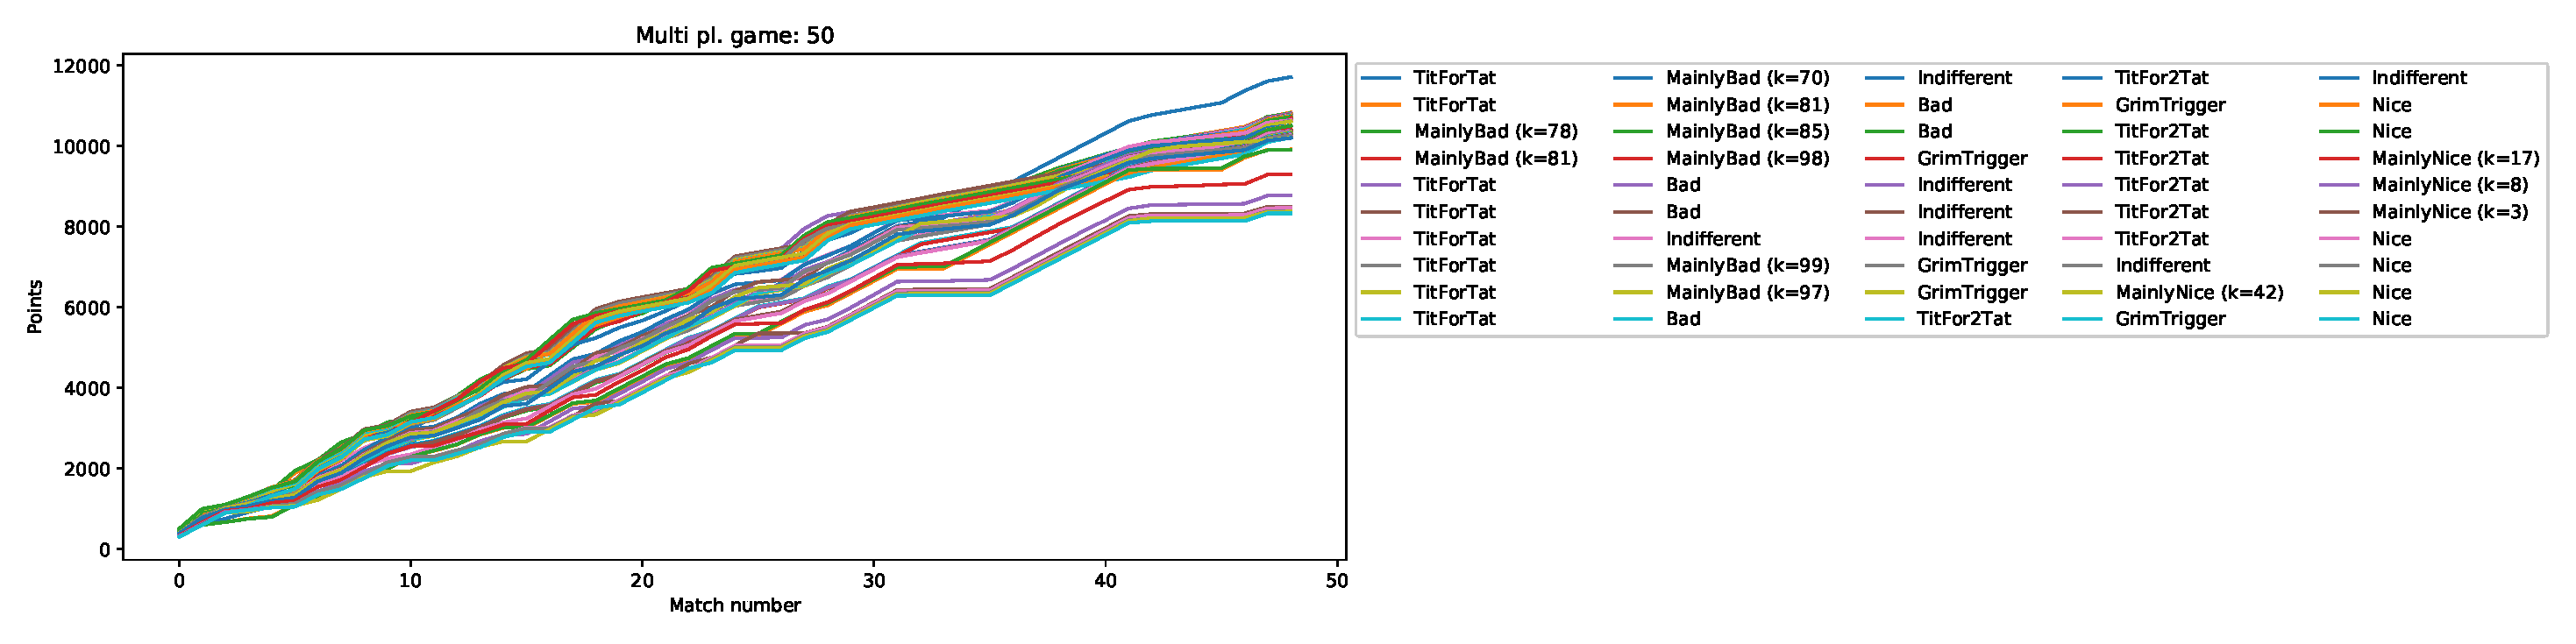
\includegraphics[width=1\columnwidth]{../img/ripdmp-const/ripdmp-scores-const-pop-50-r0}
    \caption{First iteration scores}
    \label{fig:constFI}
\end{figure}

\begin{figure}[!ht]
    \centering
    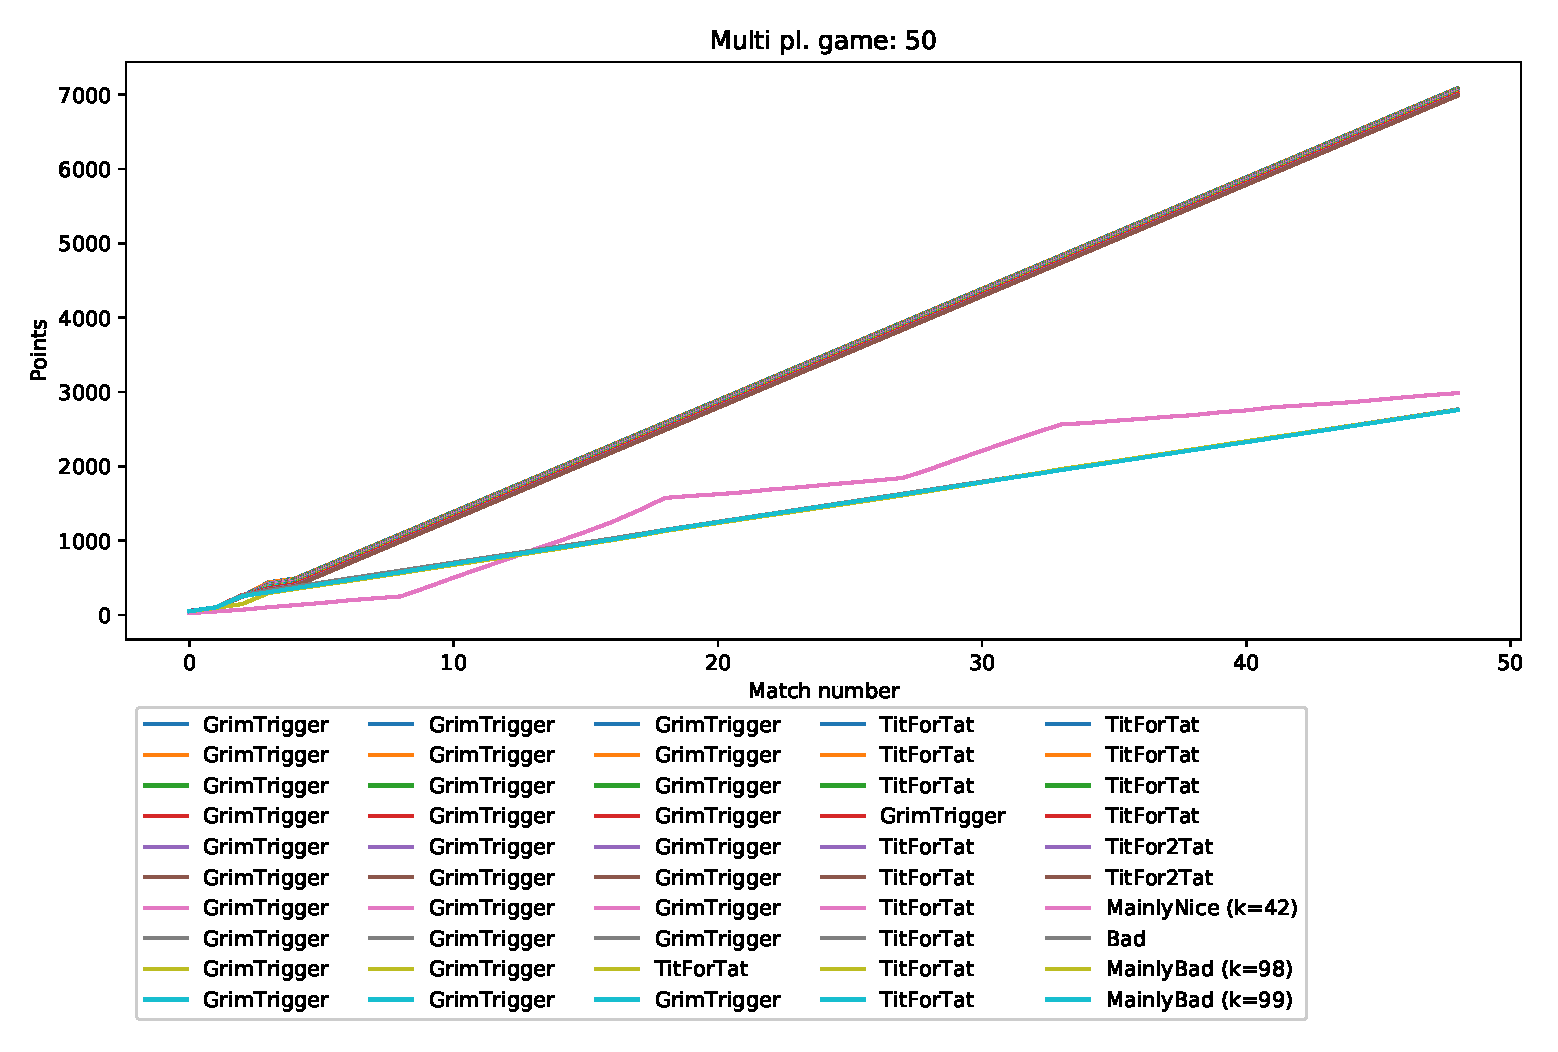
\includegraphics[width=1\columnwidth]{../img/ripdmp-const/ripdmp-scores-const-pop-50-r3}
    \caption{Last iteration scores}
    \label{fig:constLI}
\end{figure}

\textbf{ADD TABLE}

\subsection{Increasing Population 1}
In this case the number of players, so the total population, is increased at each iteration. After the round each player has a probability based on his ranking to, lets say, have a child of the same type; this probability can be expressed by $p(i)=1-\frac{i}{\#Number\ of\ players}$ where $i$ is the position reached. So the winner of the round is certain to be doubled($p(0)=1$), while the looser is certain to be not($p(last)=0$).
For each player we draw a random number, accordingly to a uniform distribution, and compare it with this probability, if we are over it we effectively double it, otherwise we do not.

\begin{figure}[!ht]
    \centering
    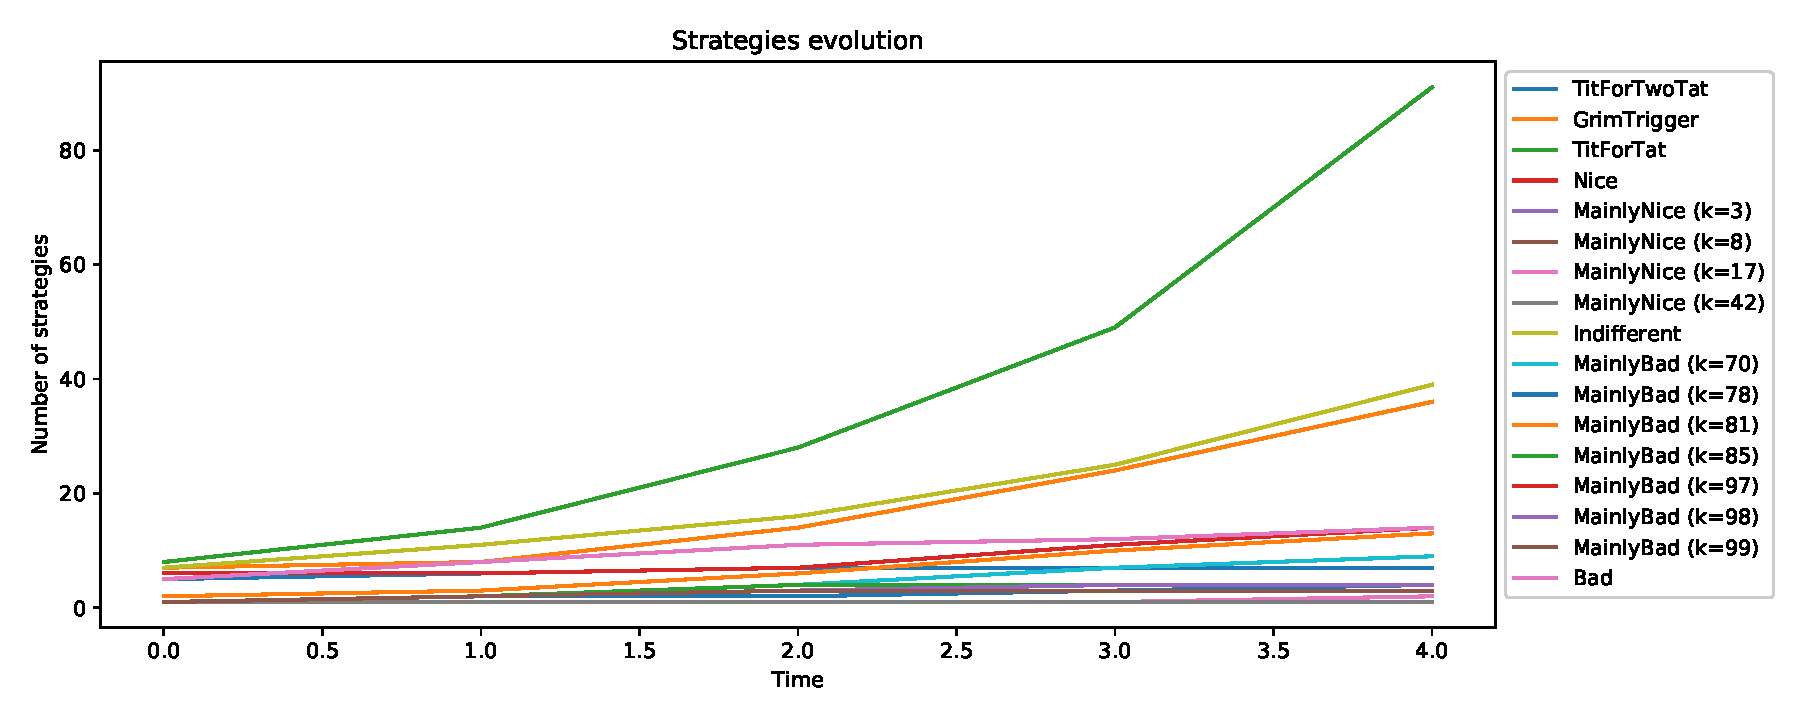
\includegraphics[width=1\columnwidth]{../img/ripdmp-incr/ripdmp-evolution-increasing-pop-50}
    \caption{Evolution RIPDMP increasing population 1}
    \label{fig:incrR}
\end{figure}

\begin{figure}[!ht]
    \centering
    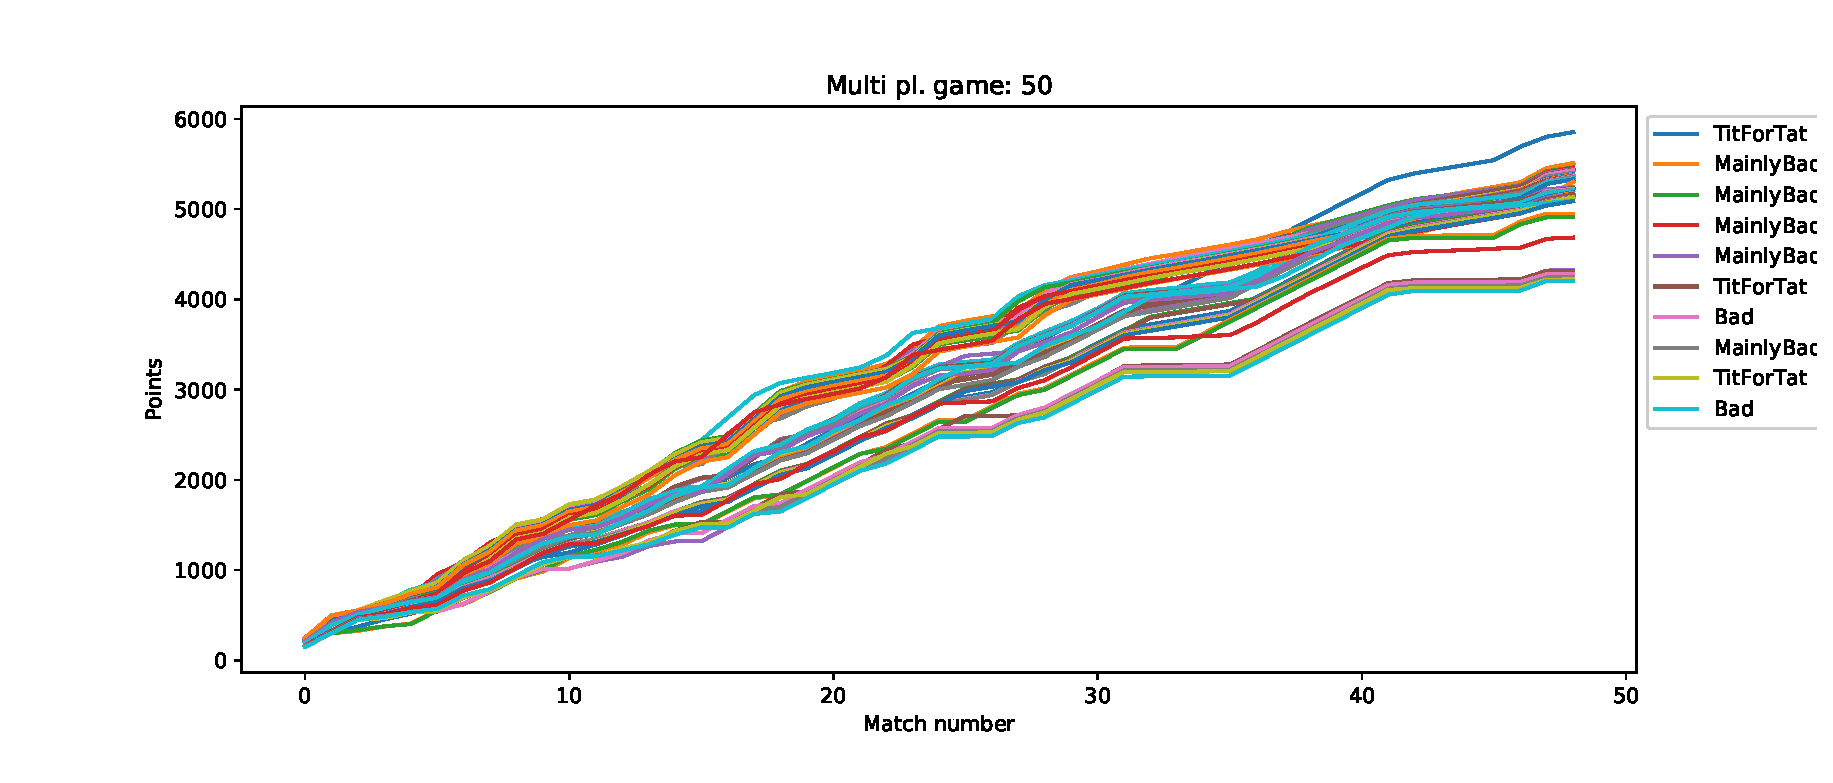
\includegraphics[width=1\columnwidth]{../img/ripdmp-incr/ripdmp-scores-increasing-pop-50-r0}
    \caption{First iteration scores}
    \label{fig:incrFI}
\end{figure}

\begin{figure}[!ht]
    \centering
    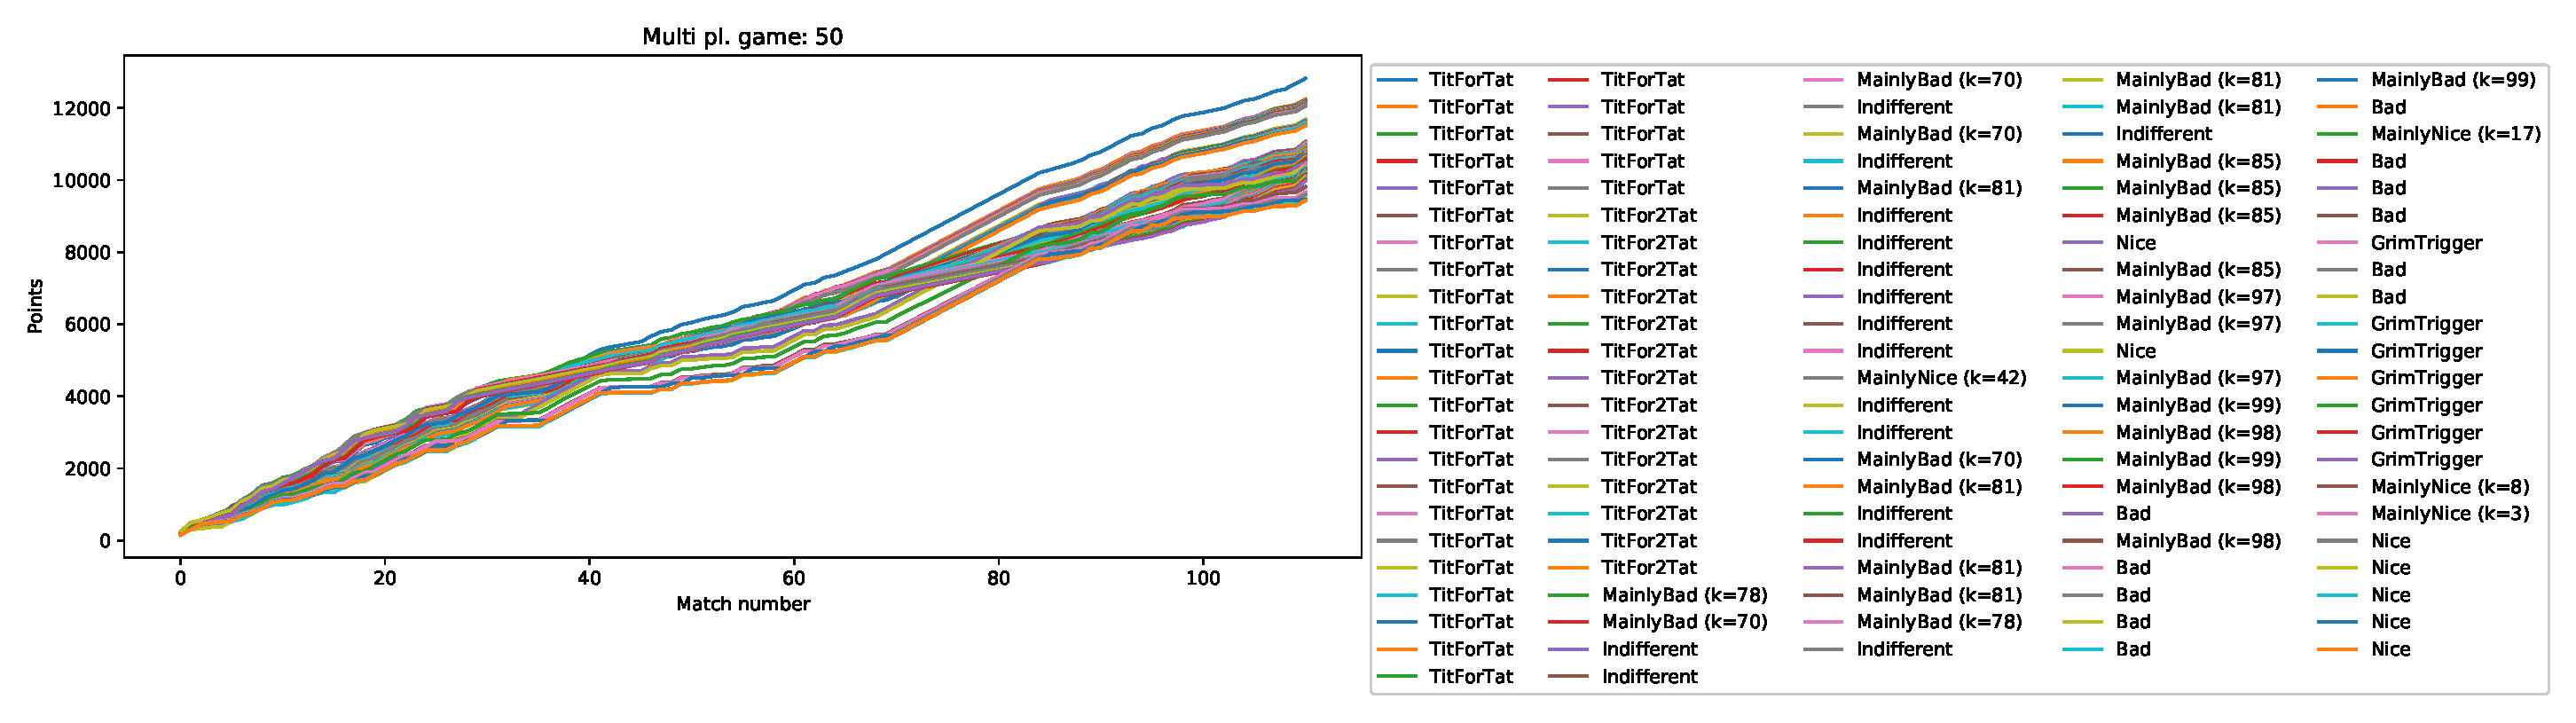
\includegraphics[width=1\columnwidth]{../img/ripdmp-incr/ripdmp-scores-increasing-pop-50-r2}
    \caption{Middle iteration scores}
    \label{fig:incrMI}
\end{figure}

\begin{figure}[!ht]
    \centering
    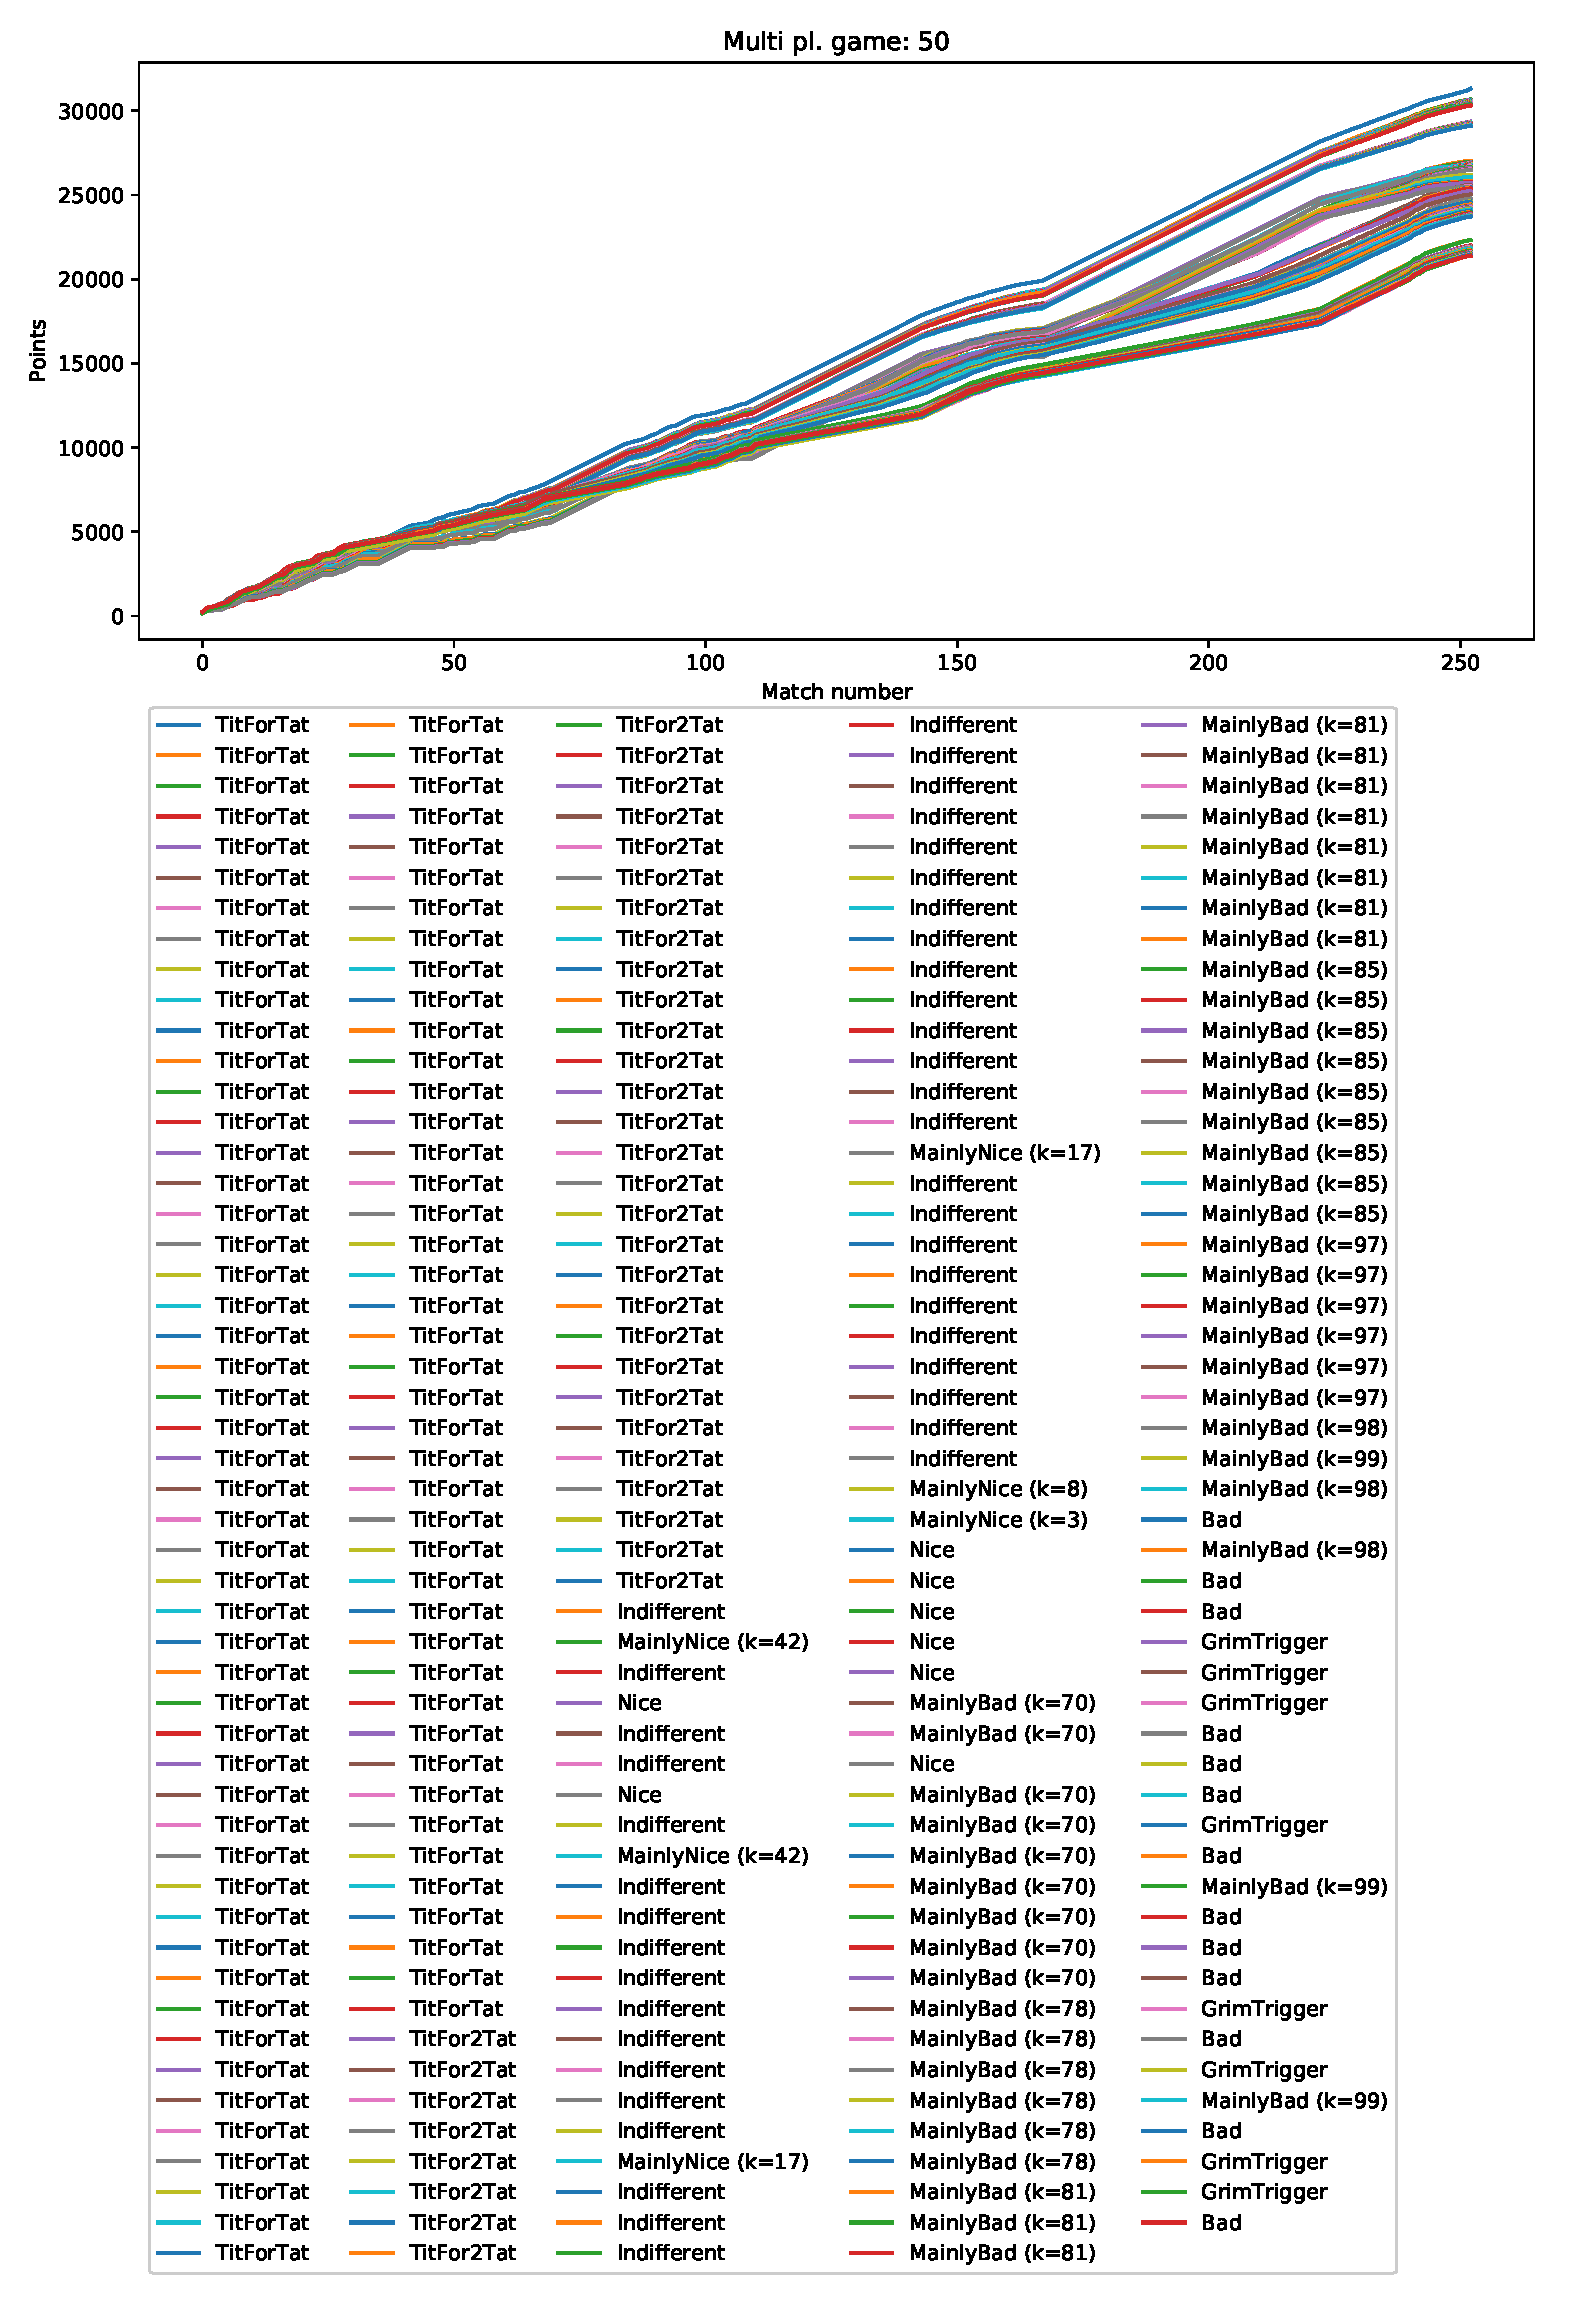
\includegraphics[width=1\columnwidth]{../img/ripdmp-incr/ripdmp-scores-increasing-pop-50-r4}
    \caption{Last iteration scores}
    \label{fig:incrLI}
\end{figure}

In this case we do not have convergence at the fifth iteration but still the simulation exhibit the same behaviour. The \textit{TfT} strategy is getting stronger and stronger. We can conclude that in the future(some more iterations), the population will converge to that.

\textbf{ADD TABLE}

\subsection{Increasing Population 2}
\textbf{TO BE COMPLETED I DO NOT KNOW THIS}

\textbf{ADD TABLE}

\textbf{ADD FIGURES}

\section{Changing rMPIPD - RR scheme} \label{s:crIPDMP}
\textbf{STILL DEVELOPING}

\section{Conclusion} \label{s:conc}

\FR{Mention the results shall be comparable with the paper.}

\balance
%\bibliographystyle{IEEEtran}
%\bibliography{report}
\end{document}
